I % Chapter 4

\chapter{Methodology} % Main chapter title
% IMPORTANT: uncomment the section enclosed by "%%%%%%%%%%%%%%%%%%%%%"
% for final document

\label{Chapter4} % For referencing the chapter elsewhere, use \ref{Chapter1} 

\lhead{Chapter 4. \emph{Methodology}} % This is for the header on each page - perhaps a shortened title

%----------------------------------------------------------------------------------------
\section{Overview}
The Dynamic Energy Map is created for a conceptual urban environment
with the following properties:
\begin{enumerate}[i.]
\item Of realistic building density and land use pattern.
  
  To achieve this, the current study used a redevelopment project at
  Lower Hill District, Pittsburgh, PA~\cite{Ramesh2013} as a
  prototype.  The land use of the conceptual urban environment is
  created based on extracted topological patterns from this
  redevelopment project.

\item The number of buildings in the model represents a typical
  community that can be served by a district energy
  system~\cite{IDEA2012}.
  
  To achieve this, the original model created under criteria i. is
  duplicated and thus there are in total 68 buildings within the
  community. It is within the range of a typical district energy
  system service capacity of 50 to 150~\cite{IDEA2012}.

\end{enumerate}

The inputs to the dynamic energy map include the hourly energy
consumption data and the urban environment layout. For the conceptual
setting, the energy data is retrieved from the simulation of DOE
Prototype buildings of new construction which comply with ASHRAE
90.1-2013 Standard~\cite{DOEprototype}.

The output of the dynamic energy map is a sequence of 2D or 3D energy
choropleth map images.

An interface is designed to provide an interactive inspection of the
map image sequence and the corresponding energy data plot of a single
buildings, building groups and the community that assists:
\begin{enumerate}[i.]
\item Comparing heating and cooling demand to identify energy recovery
  opportunities
\item Comparing heating and electricity demand to size a co-generation
  system
\end{enumerate}

\begin{figure}[h!]
  \centering
  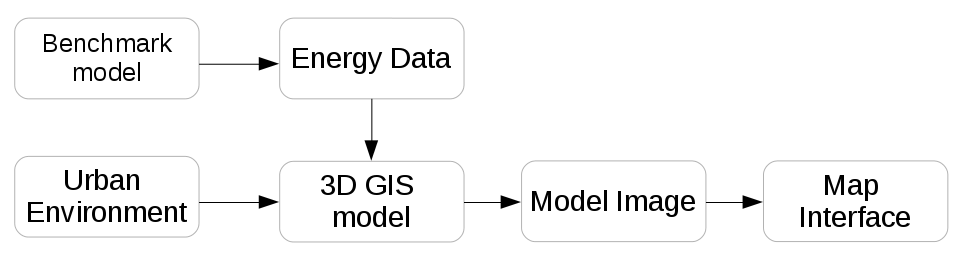
\includegraphics[width=0.7\linewidth]{flow.png}
  \caption[General Work Flow]{General Work Flow}
  \label{fig:flow}
\end{figure}

Details in input output data and the interface design process will be
explained in more details in the following sections.
\newpage
\section{Input}
\subsection{Prototype Models and Energy Data}
In the Lower Hill District project, the Commercial Prototype Building
Models (ASHRAE90.1-2013)~\cite{DOEprototype} developed by the U.S.
Department of Energy (DOE) were used to represent buildings in the
community model in the district energy system feasibility
analysis. This approach allows for a fast initial assessment of the
district system~\cite{baird2014}.

Following the same approach, the energy profile used in the current
study is retrieved from simulation results of commercial prototype
building buildings developed by U.S. Department of Energy
(DOE)~\cite{DOEprototype}. There are 16 building types in the prototype
models (\fref{tab:doeModel}). The building types involved in the
current project include: the Large Office (LO), the Medium Office (MO), Small
Office (SO), Stand-alone Retail (SR), Strip Mall (SM), the Quick Service
Restaurant (QR), Full Service Restaurant (FR), the Large Hotel (LH) and
the Midrise Apartment (MA). The two-letter shorthand in the parenthesis
after each building type is used in the building label for the dynamic
map display. The general information for the prototype buildings are
shown in \tref{tab:doeModel}:

\begin{table}[h!]
  \centering
  \begin{tabular}{l|r|r}
    \hline
Building Type                & Building Area/ft2 & Number of Floors\\
    \hline
Small Office                 & 5502              & 1\\
Medium Office                & 53628             & 3\\
Large Office                 & 498588            & 12\\
Stand-alone Retail           & 24692             & 1\\
Strip Mall                   & 22500             & 1\\
Primary School               & 73959             & 1\\
Secondary School             & 210886            & 2\\
Outpatient Healthcare        & 40946             & 3\\
Hospital                     & 241501            & 5\\
Small Hotel                  & 43202             & 4\\
Large Hotel                  & 122120            & 6\\
Warehouse (non-refrigerated) & 52045             & 1\\
Quick Service Restaurant     & 2501              & 1\\
Full Service Restaurant      & 5502              & 1\\
Mid-rise Apartment           & 33741             & 4\\
High-rise Apartment          & 84351             & 10\\
    \hline
\end{tabular}
\caption{DOE Prototype Building General Information~\cite{DOE2015}}
\label{tab:doeModel}
\end{table}

The prototype buildings comply with the ASHRAE Standard 90.1-2013. The
HVAC system types are shown in \tref{tab:hvac}. The major heating
systems of the prototype buildings are gas furnace and boilers. Some
are with packed terminal air conditioner as backup system. The two
exceptions are the Small Office and the High-rise Apartment. The
former uses an air-source heat pump for space heating with a gas
furnace as backup. The latter uses a water source heat pump for space
heating. The cooling system for most building types are packaged air
conditioning unit. The Large Office, the Secondary School, the Hospital
and Large Hotel use air or water-cooled chillers. The Small Office and
the High-rise Apartment use water source heat pump for space cooling.

\pagebreak
\begin{table}[h!]
\centering
%\scriptsize
\tiny
\caption{Prototype Building HVAC System}
\label{tab:hvac}
%\begin{tabular}{l|p{3cm}|p{4cm}|p{4cm}}
\begin{longtable}{p{2cm}|p{2cm}|p{4cm}|p{4cm}}
  \hline
  Building Type                & Heating                                                                         & Cooling                                                                      & Air                                                                                                                                                                    \\
  \hline
  \hline
  Small Office                 & Air-source heat pump with gas furnace as back up                                & Air-source heat pump                                                         & Single zone, constant air volume air distribution, one unit per occupied thermal zone                                                                                  \\
  \hline
  Medium Office                & Gas furnace inside the packaged air conditioning unit                           & Packaged air conditioning unit                                               & VAV terminal box with damper and electric reheating coil                                                                                                               \\
  \hline
  Large Office                 & Gas boiler                                                                      & Water-source direct expansion cooling coil with fluid cooler for datacenter and IT closets & VAV terminal box with damper and hot-water reheating coil                                                                                                              \\
                               &                                                                                 & Two water-cooled centrifugal chillers for the rest of the building           & non-datacenter portion of the basement and IT closets that are served by CAV units.                                                                                    \\
  \hline
  Stand-alone Retail           & Standalone gas furnace for front\_entry                                         & Packaged air conditioning unit                                               & Constant air volume air distribution                                                                                                                                   \\ & Gas furnace inside the packaged air conditioning unit for the rest              &                                                                              &                                                                                                                                                                        \\
  \hline
  Strip Mall                   & Gas furnace inside the packaged air conditioning unit                           & Packaged air conditioning unit                                               & single-zone rooftop units with Constant air volume air distribution                                                                                                    \\
  \hline
  Primary School               & 1. Gas furnace inside packaged air conditioning unit                            & Packaged air conditioning unit                                               & 1. CAV systems: direct air from the packaged air conditioning unit                                                                                                     \\
                               & 2. Hot water from a gas boiler for heating                                      &                                                                              & 2. VAV systems: VAV terminal box with damper and hot water reheating coil                                                                                              \\
  \hline
  Secondary School             & 1. Gas furnaces inside packaged air conditioning units                          & 1. Packaged air conditioner                                                  & 1. CAV system: direct air from the packaged unit                                                                                                                       \\
                               & 2. Gas-fired boiler  provide heating hot water and chilled water to these AHUs. & 2. Air-cooled Chiller                                                        & 2. VAV System: VAV terminal box with damper and hot water reheating coil                                                                                               \\
  \hline
  Outpatient Healthcare        & Gas boiler                                                                      & direct expansion cooling coil                                                              & VAV terminal box with damper and hot water reheating coil                                                                                                              \\
  \hline
  Hospital                     & Gas boiler                                                                      & Two water cooled centrifugal chiller                                         & Medical critical zones: variable air volume systems with hot water reheating and electric stream humidifiers.                                                          \\
                               &                                                                                 &                                                                              & Non-critical zones: VAV systems for general zones and one constant air volume (CAV) system for kitchen zone: VAV terminal box with damper and hot water reheating coil \\
  \hline
  Small Hotel                  & Guest rooms:  Packed terminal air conditioner with electric resistance heating  & Guest rooms and corridors:  Packed terminal air conditioner                  & Constant air volume systems                                                                                                                                            \\
                               & Public spaces:  gas furnace inside the packaged air conditioning units          & Public space:  Split system with direct expansion cooling                                  &                                                                                                                                                                        \\
                               & Storage and stairs: electric cabinet heaters                                    &                                                                              &                                                                                                                                                                        \\
  \hline
  Large Hotel                  & One gas-fired boiler                                                            & One air-cooled chiller                                                       & Public spaces on ground floor and top floor: VAV with hot water reheating coils;                                                                                       \\
                               &                                                                                 &                                                                              & Guest Rooms:  dedicated outside air system + four-pipe fan-coil units.                                                                                                 \\
  \hline
  Warehouse (non-refrigerated) & Gas furnace inside the packaged air conditioning unit                           & Packaged air conditioning unit                                               & Direct, uncontrolled air                                                                                                                                               \\
  \hline
  Quick Service Restaurant     & Gas furnace inside the packaged air conditioning unit                           & Packaged air conditioning unit                                               & Single zone, constant air volume air distribution                                                                                                                      \\
  \hline
  Full Service Restaurant      & Gas furnace inside the packaged air conditioning unit                           & Packaged air conditioning unit                                               & Single zone, constant air volume air distribution                                                                                                                      \\
  \hline
  Mid-rise Apartment           & Gas Furnace                                                                     & Split system direct expansion (1 per apt)                                                  & Constant volume                                                                                                                                                        \\
  \hline
  High-rise Apartment          & Water Source Heat Pumps                                                         & Water Source Heat Pumps                                                      & Constant volume                                                                                                                                                      \\ 
  \hline
\end{longtable}
\end{table}

\pagebreak
\subsubsection{Input for Identifing Energy Recovery
  Opportunities}\label{sec:inputRecover}
The major heat rejection sources include heating mode heat rejection
and cooling mode heat rejection. The heat rejection in heating mode
happens during the process of the mixing of conditioned and outside
air. This source of heat rejection is more difficult to capture and is
thus left out from the energy recovery potential calculation in this
study. The current study will only focus on the cooling induced heat
reject. 

The heat rejection in cooling mode happens during the condensing
process when the high temperature refrigerant gas condenses or in the
condenser loop by evaporative cooling~\cite{Bhatia2015}:
\begin{itemize}
\item Air cooled unit: ambient air is blown through condensing coils
  and removes heat from the gas refrigerant.
\item Water cooled chiller with cooling tower: A water-cooled chiller
  removes heat and reject the heat to the condenser water loop. The
  condenser water loop contains a cooling tower and the heat in the
  condenser water loop is rejected to the outside through
  evaporation~\cite{coolingTower2015}.
\item Water cooled fluid cooler: water is sprayed on the condensing
  coil with fan forced air flowing in the opposite direction. It
  causes evaporative cooling effect that takes away the heat from the
  gas refrigerant.
\end{itemize}
The ``condenser total heat of rejection''~\cite{Bhatia2015} (THR) in
the condensing process equals to the ``net refrigeration effect''
~\cite{Bhatia2015}(RE, the hourly cooling demand), plus the compressor
input, it can be represented with the following equation~\cite{Bhatia2015}:

\begin{equation}\label{eq:reject}
THR = RE * f 
\end{equation}

$f$ is the ``Heat Rejection Factor'' and it is typically between 1.15
and 1.25~\cite{Bhatia2015}. The water-based system has heat rejection
factor closer to 1.15 and the air-based system closer to
1.25~\cite{Bhatia2015}.

To help users identify energy recovery opportunities, the energy
information needed to retrieve include: space heating energy demand
and space cooling energy demand. The space cooling demand (RE in
\eref{eq:reject}) is an indicator for heat rejection that could be
recovered and shared within a single building or a building group. The
heat rejection that could be captured and reused by the building that
produces reject heat or by nearby buildings is very complicated and
involves the detailed configurations of the cooling system, cooling
energy transmission system and the energy recovery system. In my
dynamic energy map for the current stage, for demonstration purpose, a
simplified assumptions is made that 100\% of the cooling reject heat
can be recovered. Thus the researcher use THR as an approximation for recoverable
cooling produced reject heat and is used in the calculation of energy
recovery potential (\sref{eq:recover}).

From \tref{tab:heatFuel}, the Small Office, the Medium Office, the Large Office,
the Outpatient Healthcare, the Hospital, the Small Hotel and the High-rise Apartment
use both electricity and natural gas for space heating, the rest of
the building types uses only natural gas for space heating. The researcher thus use
the EnergyPlus simulation output parameters ``heating:electricity''
and ``heating:gas'' to represent the space heating demand of reference
buildings.
\begin{table}[h]
\centering
\caption{Annual Total Heating Demand by Fuel Type~\cite{DOE2015}}
\label{tab:heatFuel}
\begin{tabular}{lrr}
  \hline
  Building Type                & Electricity {[}kBtu{]} & Natural Gas {[}kBtu{]} \\
  \hline
  \hline
  
  Small Office                 & 8189.1                 & 5658.5                 \\
  Medium Office                & 197799.9               & 264213.5               \\
  Large Office                 & 10236.4                & 5047893.3              \\
  Stand-alone Retail           & 0                      & 172550.1               \\
  Strip Mall                   & 0                      & 525450.8               \\
  Primary School               & 0                      & 1099012.8              \\
  Secondary School             & 0                      & 813350.2               \\
  Outpatient Healthcare        & 290458.5               & 472230.9               \\
  Hospital                     & 805606.5               & 6794103.9              \\
  Small Hotel                  & 266061.7               & 112117.3               \\
  Large Hotel                  & 0                      & 1831627.9              \\
  Warehouse (non-refrigerated) & 0                      & 645141.1               \\
  Quick Service Restaurant     & 0                      & 545838.3               \\
  Full Service Restaurant      & 0                      & 749543.2               \\
  Mid-rise Apartment           & 0                      & 375307.1               \\
  High-rise Apartment          & 229712.9               & 831605.2               \\
  \hline
\end{tabular}
\end{table}

\begin{figure}[h!]
  \centering
  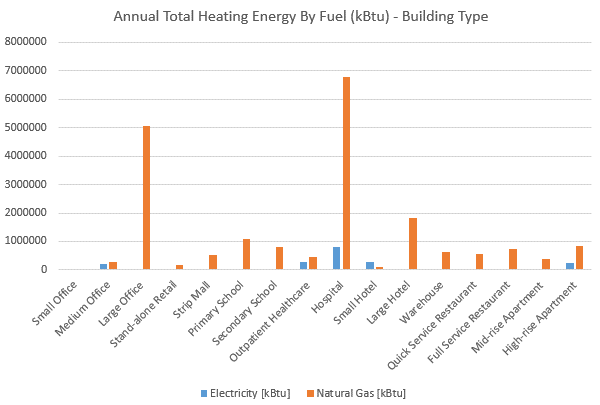
\includegraphics[width=0.7\linewidth]{heatFuel.png}
  \caption[Heating Fuel]{Heating Fuel}
  \label{fig:heatFuel}
\end{figure}

Electricity is the only fuel used for space cooling~\cite{DOE2015},
thus the EnergyPlus output parameter ``cooling:electricity'' is used
to represent space cooling demand. According to the suggested heat
rejection factor~\cite{Bhatia2015}, the heat recovery potential will
be calculated with $f = 1.15$ for the Large Office, the Hospital and the High-rise
Apartment, and $f = 1.25$ for the remaining building types:
\begin{equation}\label{eq:recover}
\text{Heat Recovery Potential} = \text{cooling:electricity} \times f
\end{equation}

In summary, to facilitate identification of energy recovery
opportunities for single buildings and within building groups, the
hourly ``heating:electricity'', ``heating:gas'' and
``cooling:electricity'' output will be extracted from EnergyPlus
simulation of all 16 DOE Commercial prototype buildings.

\subsubsection{Input for Sizing District Co-generation
  System}
For the sizing of a district co-generation system, the relevant
information needed are the total heating demand, and the total
electricity demand. The general principle used in Lower Hill District
project ~\cite{baird2014} is to use the minimum total heat demand
(space heating and service hot water) over time to assess the minimum
capacity of electricity generation ($E_{heat}$) such that its heat
bi-product from electricity generation will always be consumed. The
maximum total electricity demand ($E_{elec}$) is used for assessing
the capacity of a backup system or a second phase system development
by $C_{backup} = E_{elec} - E_{heat}$ where $C_{backup}$ is the
capacity of electricity generation for the backup system or
second-phase development.

Heating demand assessed in the sizing of co-generation system is
different from the energy recovery use case in \sref{sec:inputRecover}
.  It contains the space heating demand and the service hot water
demand. From the summary files of prototype models, one can observe
that the Small Office, Strip Mall, Warehouse and Mid-rise Apartment use
electricity to produce service hot water; the Medium Office, the Large Office,
Stand-alone Retail, the Outpatient Healthcare, the Small Hotel, the Quick Service
Restaurant and the High-rise Apartment use gas for service hot water;
Primary School, the Secondary School, the Hospital, the Large Hotel and Full
Service Restaurant use both electricity and gas for service hot water
(\tref{tab:hotWater}). Thus the variable ``Water
Heater:WaterSystems:Electricity'' and ``Water
Heater:WaterSystems:Gas'' are used for representing energy demand for
service hot water.

The output parameter ``electricity:facility'' was extracted to
represent the total electricity demand.

\begin{table}[h!]
\centering
\caption{Service Hot Water by Fuel Type}
\label{tab:hotWater}
\begin{tabular}{l|r|r}
  \hline
Building Type                & Electricity {[}kBtu{]} & Natural Gas {[}kBtu{]} \\
  \hline
  \hline
Small Office                 & 17070.2                & 0                      \\
Medium Office                & 0                      & 76090.7                \\
Large Office                 & 0                      & 543231.8               \\
Stand-alone Retail           & 0                      & 91113.6                \\
Strip Mall                   & 61475.4                & 0                      \\
Primary School               & 24491.6                & 119823                 \\
Secondary School             & 146352.4               & 501006.6               \\
Outpatient Healthcare        & 0                      & 126524.1               \\
Hospital                     & 25098.2                & 1199178.1              \\
Small Hotel                  & 0                      & 603797.3               \\
Large Hotel                  & 86004.9                & 2050241.9              \\
Warehouse (non-refrigerated) & 24719.1                & 0                      \\
Quick Service Restaurant     & 0                      & 188473.4               \\
Full Service Restaurant      & 71550.7                & 326902.1               \\
Mid-rise Apartment           & 394917.4               & 0                      \\
High-rise Apartment          & 0                      & 1116452.6              \\
  \hline
\end{tabular}
\end{table}

\pagebreak
\subsection{Simulation Data Analysis of the prototype
  models}\label{boxPlot}
The output of EnergyPlus simulation of 16 prototype buildings are
read, processed and plotted with a Python program. The data loading
and processing utility is used in both data analysis and the dynamic
plot in the interface design.

The energy output retrieved from EnergyPlus includes ``Heating:Gas'',
``Heating:Electricity'', ``Cooling:Electricity'', ``Water
Heater:WaterSystems:Gas'', ``Water Heater:WaterSystems:Electricity''
and ``Electricity:Facility''. This section will include some basic
aggregated analysis of the data distribution.  The meaning of each
output variable is listed in \tref{tab:outputMeaning}:
\begin{table}[h!]
\centering
\caption{Table of EnergyPlus output and their meaning}
\label{tab:outputMeaning}
\begin{tabular}{l|l}
  \hline
  EnergyPlus Output            & Meaning\\
  \hline
  \hline
  Heating:Gas                  & Total gas for space heating         \\
  Heating:Electricity          & Total electricity for space heating \\
  Water Heater:WaterSystem:Gas & Total gas for service hot water     \\
  Water Heater:WaterSystem:Electricity & Total Electricity for service hot water     \\
  Cooling:Electricity          & Total electricity for space cooling \\
  Electricity:Facility         & Total electricity                  \\
  \hline
\end{tabular}
\end{table}

\subsubsection{Single Output}
Analyzing the EnergyPlus ~\cite{EnergyPlus2015} simulation result of
the output above provides a basic understanding of the energy profile
data distribution involved in the current project. This can be used as
a basis to compare with the additional analysis one can perform in a
dynamic energy map described in the following sections.

To analyze the general distribution of each output variable, a box
plot was created for each of the five variables. By analyzing each
single output, a great difference between different
building types was apparent.

The hourly gas heating demand of the prototype buildings ranges from 0
to 8000 kBtu/hr. The majority (75\%) of all hourly consumption is
below 1000 kBtu/hr. All building types have a large number of outliers
above the 75\% quartile. This indicates that the gas heating demand of
all building types are severely right skewed which means the median is
much smaller then the mean of the distribution and the data set has
many extremely large values. The Hospital has the highest median gas
heating demand of about 800 kBtu/hr. The Large Hotel has the second
larges hourly gas heating demand. This indicates that the Hospital and
the Large Hotel has year-round high heating demand and they can act as
anchor load buildings in a district energy system. In terms of peak
demand, The Large Office and the Secondary School have the highest
peak hourly gas heating demand (\fref{fig:HG}).
\begin{figure}[h!]
  \centering
  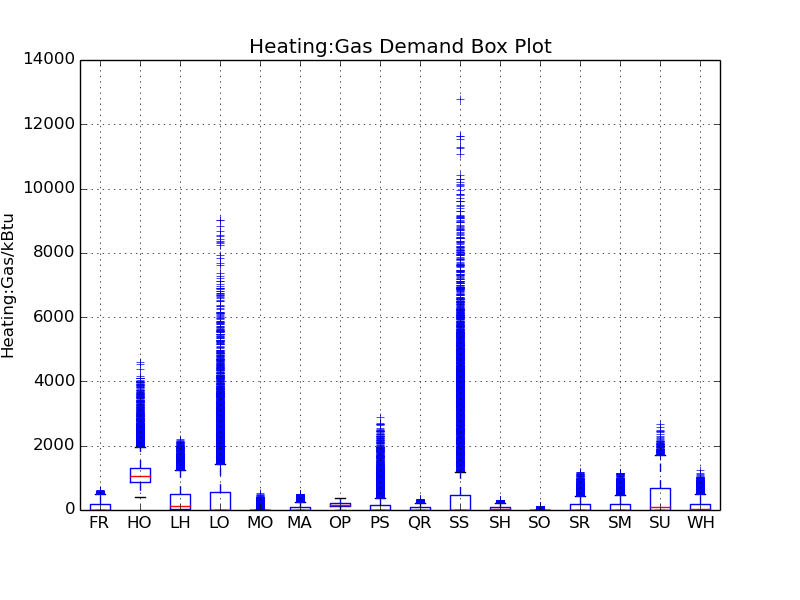
\includegraphics[width=0.7\linewidth]{HG}
  \caption[Heating:Gas Box Plot]{Heating:Gas Box Plot}
  \label{fig:HG}
\end{figure}%

The hourly hot water demand of the prototype buildings ranges from 0
to 600 kBtu/hr, about 1/12 of the range of space heating gas
demand. Most buildings have median hot water hourly demand below 150
kBtu/hr. Primary School and the Secondary School has a large number of
outliers above the 75\% quartile and the hot water demand of these two
types of buildings are severely right skewed. This means these two
building types have a lot of large values in their hot water demand
profile. The High-rise Apartment and the Large Hotel have the largest
median hot water demand of about 150 kBtu/hr, indicating that these
two building types have year round high hot water demand and they may
act as anchor load buildings in a district energy system that
distribute hot water. The First Service Restaurant, the Hospital, the
Large Office, the Mid-rise Apartment and the Small hotel all have a
median service hot water demand of about 50 kBtu/hr. The remaining
building types have almost zero median hot water demand. The Large
Hotel and the Secondary School has the highest peak demand for service
hot water. (\fref{fig:WH}).
\begin{figure}[h!]
  \centering
  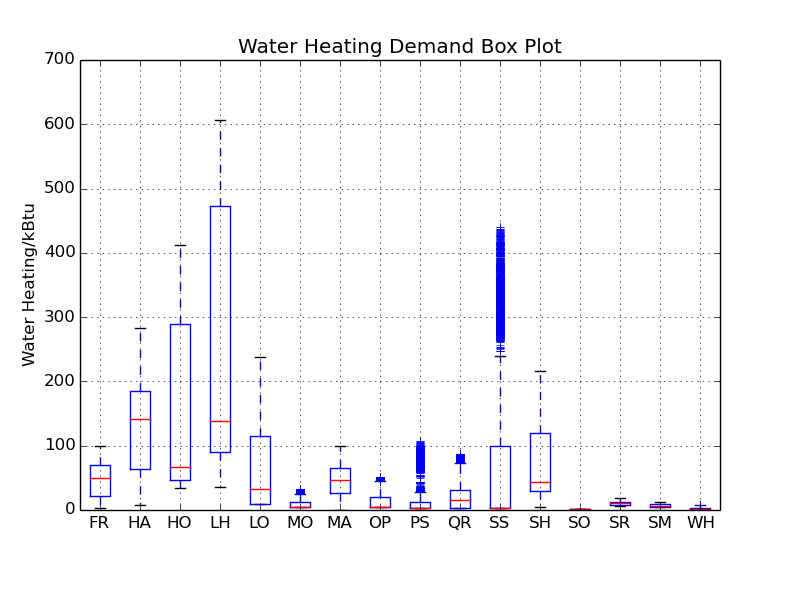
\includegraphics[width=0.7\linewidth]{WH}
  \caption[Service Hot Water Box Plot]{Service Hot Water Box Plot}
  \label{fig:WH}
\end{figure}%

\begin{figure}[h!]
  \centering
  \begin{subfigure}{0.4\textwidth}
  \centering
  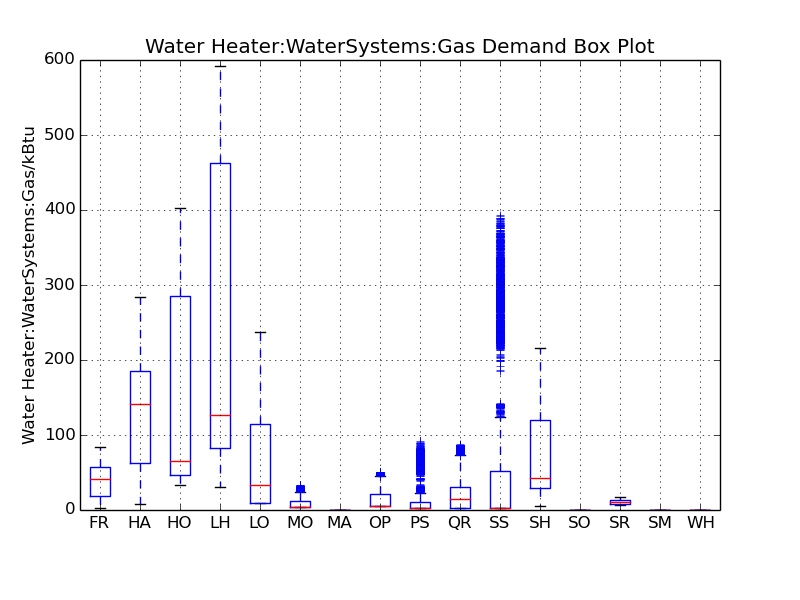
\includegraphics[width=\linewidth]{WHWSG}
  \caption[Gas Water Heating Box Plot]{Gas Water Heating Box Plot}
  \label{fig:WHWSG}
\end{subfigure}
~
\begin{subfigure}{0.4\textwidth}
  \centering
  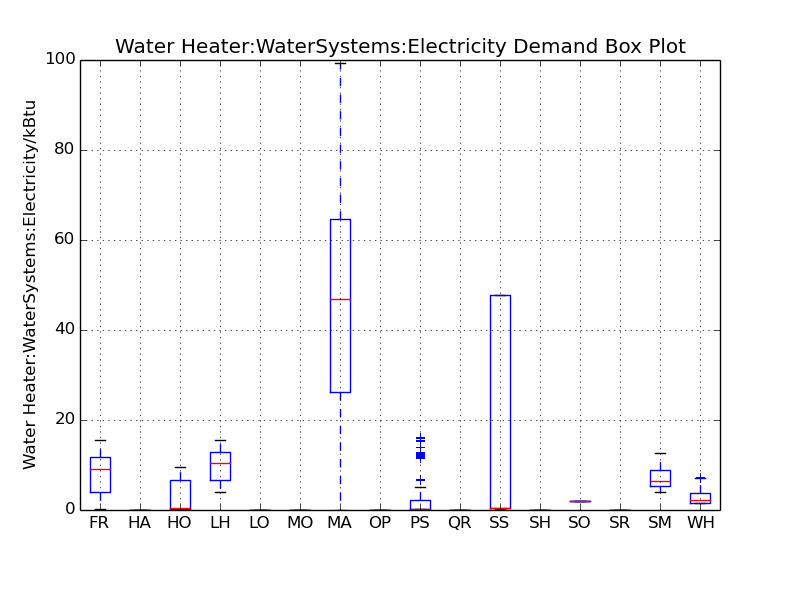
\includegraphics[width=\linewidth]{WHWSE}
  \caption[Electricity Water Heating Box Plot]{Electricity Water Heating Box Plot}
\end{subfigure}
\caption[Comparing Heating:Gas and Space Heating]{Comparing
  Heating:Gas and Space Heating}
\end{figure}

From \tref{tab:heatFuel}, the Small Office, the Medium Office, the
Large Office, the Outpatient Healthcare, the Hospital, the Small Hotel
and the High-rise Apartment use electricity and natural gas for space
heating. The hourly electricity heating demand of these buildings
ranges from about 0 to 630 kBtu/hr. Almost all of them have nearly
zero median electricity heating demand, except the median demand for
the Outpatient Healthcare is around 30 kBtu/hr. This means the
electricity space heating equipment only operates in heating seasons.
Almost all building types have a large number of outliers above the
75\% quartile except for the Hospital. The Medium Office has the
highest hourly electricity heating peak demand and the Outpatient
Healthcare and the Small Hotel have the second largest hourly
electricity heating peak demand (\fref{fig:HE}).

\begin{figure}[h!]
  \centering
  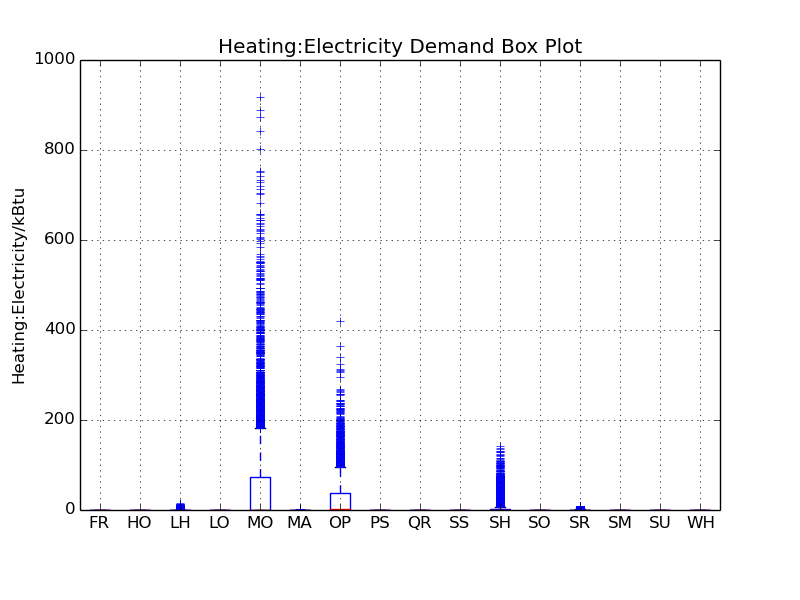
\includegraphics[width=0.7\linewidth]{HE}
  \caption[Heating:Electricity Box Plot]{Heating:Electricity Box Plot}
  \label{fig:HE}
\end{figure}% 

The hourly cooling demand among the prototype building types ranges
from 0 to 2000 kBtu/hr, which is about 25\% of that of the peak gas
heating demand. The Hospital has the largest median cooling demand of
about 150 kBtu/hr. All building types have a large number of outliers
above the 75\% quartile, indicating a severe right skew for their
hourly cooling demand distribution. This indicates there are a lot
large values in their demand profile.  The building types with zero
median hourly cooling demand then require cooling only in the cooling
season. In terms of hourly cooling peak demand, the Large Office has
the highest peak demand of about 1900 kBtu/hr and the Secondary School
has the second largest peak demand of about 1500 kBtu/hr. There are
five building types with non-zero median hourly cooling demand: the
Hospital, the Large Office, the Outpatient Health Care, the Large
Hotel and the Small Hotel. This means they need space cooling for at
least 50\% of the year. The constant cooling demand creates
opportunities for energy recovery of reject heat produced by space
cooling (\fref{fig:CE}).
\begin{figure}[h!]
  \centering
  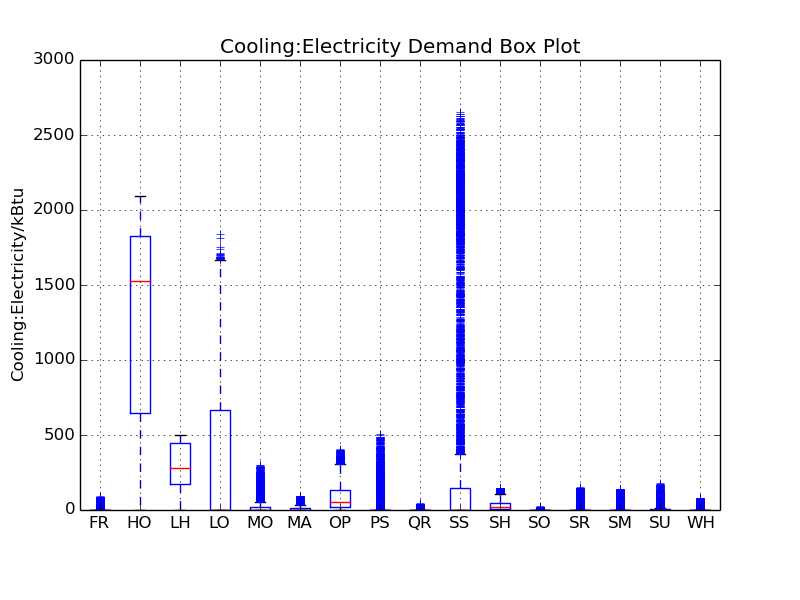
\includegraphics[width=0.7\linewidth]{CE}
  \caption[Cooling:Electricity Box Plot]{Cooling:Electricity Box Plot}
  \label{fig:CE}
\end{figure}%

The hourly electricity demand of prototype buildings ranges from 0 to
8000 kBtu/hr, which is about the same as that of the peak gas heating
demand. Comparing with other output variables, the electricity demand
distribution has fewer outliers in general. This indicates that all
building types have consistent electricity demand all year
round. There are not as many extremely large demand values in the
electricity demand profile of any building type. The Large Office
has the largest median hourly electricity demand (about 3400
kBtu/hr). The Hospital has the second largest median hourly
electricity demand (about 2000 kBtu/hr). The Large Office has the
largest electricity hourly peak demand.

\begin{figure}[h!]
  \centering
  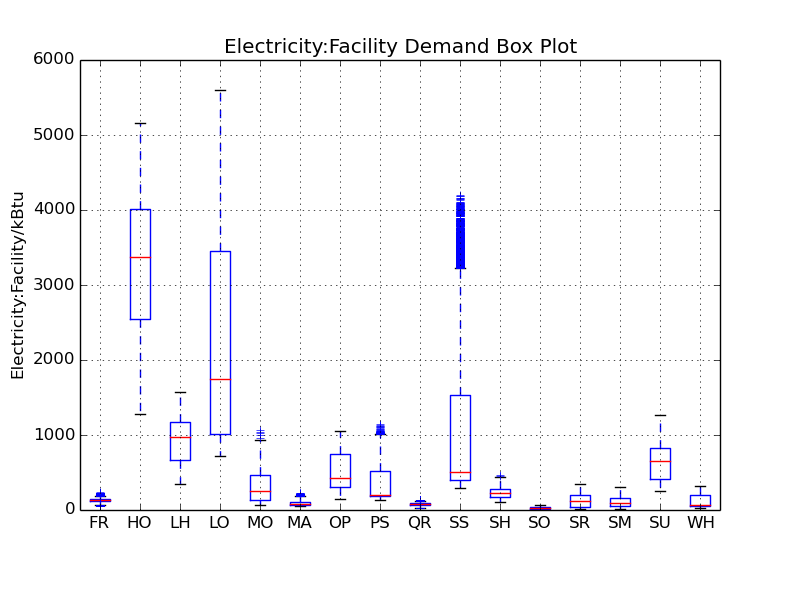
\includegraphics[width=0.7\linewidth]{EF}
  \caption[Electricity:Facility Box Plot]{Electricity:Facility Box
    Plot}
  \label{fig:EF}
\end{figure}%

\subsubsection{Space Heating Demand vs. Space Cooling Demand}
The hourly space heating demand of the prototype buildings closely
follows the distribution of gas heating demand, with minor demand
increase in the Hospital, the Medium Office and the Outpatient Health
Care (\fref{fig:SH}).

\begin{figure}[h!]
  \centering
  \begin{subfigure}{0.4\textwidth}
  \centering
  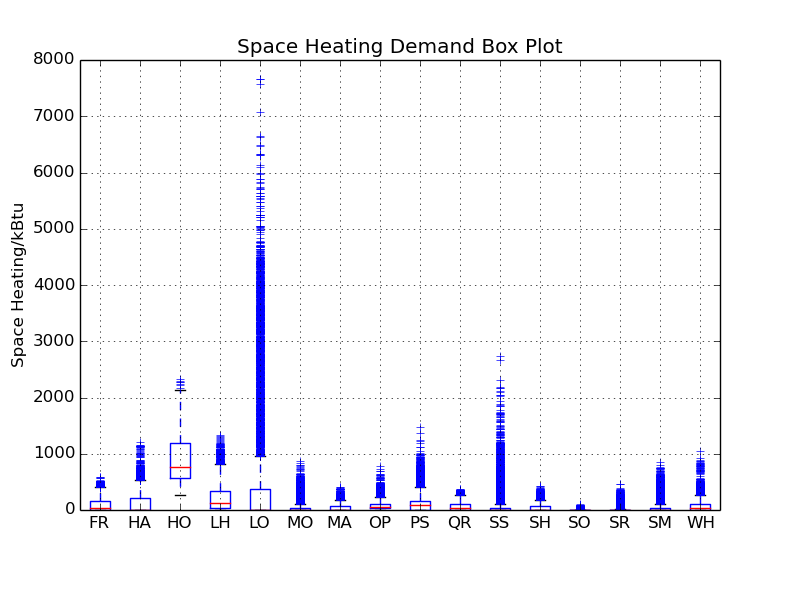
\includegraphics[width=\linewidth]{SH}
  \caption[Space Heating Demand Box Plot]{Space Heating Demand Box
    Plot}
  \label{fig:SH}
\end{subfigure}
~
\begin{subfigure}{0.4\textwidth}
  \centering
  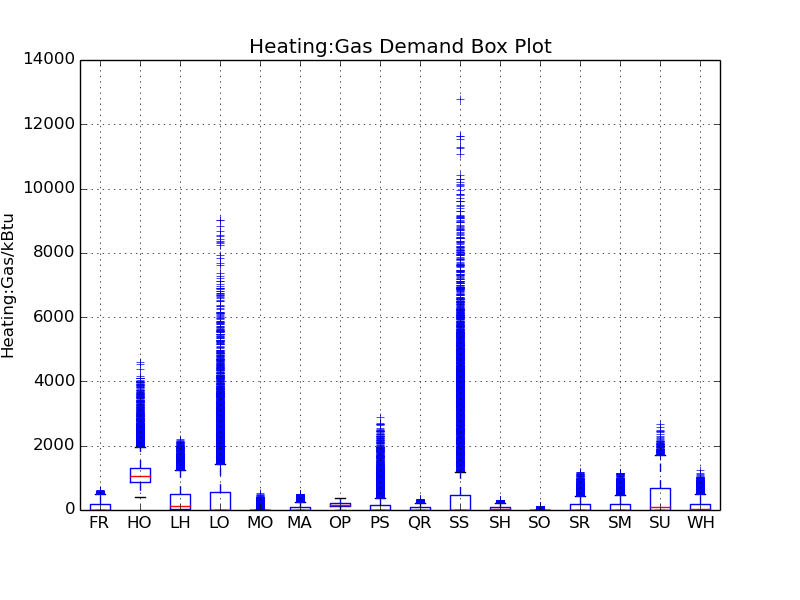
\includegraphics[width=\linewidth]{HG}
  \caption[Heating:Gas Box Plot]{Heating:Gas Box Plot}
  \label{fig:HG2}
\end{subfigure}
\caption[Comparing Heating:Gas and Space Heating]{Comparing
  Heating:Gas and Space Heating}
\end{figure}

Comparing the space heating (Heating:Gas and Heating:Electricity) with
space cooling (Cooling:Electricity), one can see that the heating peak
demand is larger than the cooling peak demand for all building
types. The Hospital, the Large Hotel and the Outpatient Health Care
have both the highest median space heating and space cooling demand,
indicating a potential for single building level energy recovery.
\begin{figure}[h!]
  \centering
  \begin{subfigure}{0.4\textwidth}
  \centering
  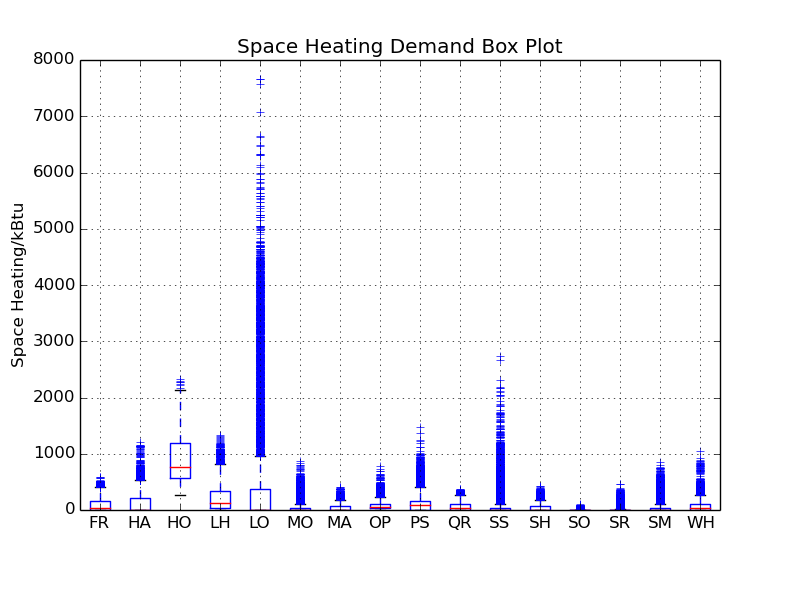
\includegraphics[width=\linewidth]{SH}
  \caption[Space Heating Demand Box Plot]{Space Heating Demand Box
    Plot}
  \label{fig:SH}
\end{subfigure}
~
\begin{subfigure}{0.4\textwidth}
  \centering
  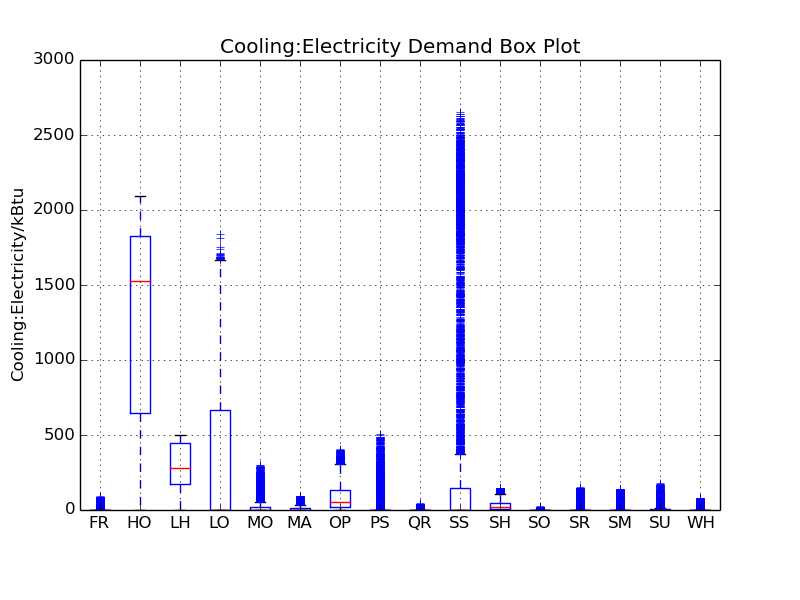
\includegraphics[width=\linewidth]{CE}
  \caption[Cooling:Electricity Box Plot]{Cooling:Electricity Box Plot}
  \label{fig:CE2}
\end{subfigure}
\caption[Comparing Space Heating and Space Cooling Demand]{Comparing
  Space Heating and Space Cooling Demand}
\end{figure}

\subsubsection{Heating Demand vs. Electricity Demand}
Comparing the heat and power demand of each prototype building type
with the ``heat to power ratio''(HTPR), one of the important
parameters of a CHP plant. Depending on the prime mover types, a CHP
plant can produce 0.6 to 10 unit of waste heat for one unit of
electricity generation~\cite{introCHP2010}. From \fref{fig:HTPR}, one
can see that the range of HTPR is from 0 to 25. The building with
highest median of HTPR is the Quick Service Restaurant (about 1.5).
The remaining building types have a median HTPR below one. Increase
the number of buildings with high HTPR ratio is helpful in increasing
the total HTPR of the community. This allows for more fully reuse of
the waste heat from power generation. In addiction, the large range of
Heat to Power ratio also indicates the necessity of heat storage
equipment that shifts the occurring time of the peak of heat demand
and electricity demand.
\begin{figure}[h!]
  \centering
  \begin{subfigure}{0.4\textwidth}
  \centering
  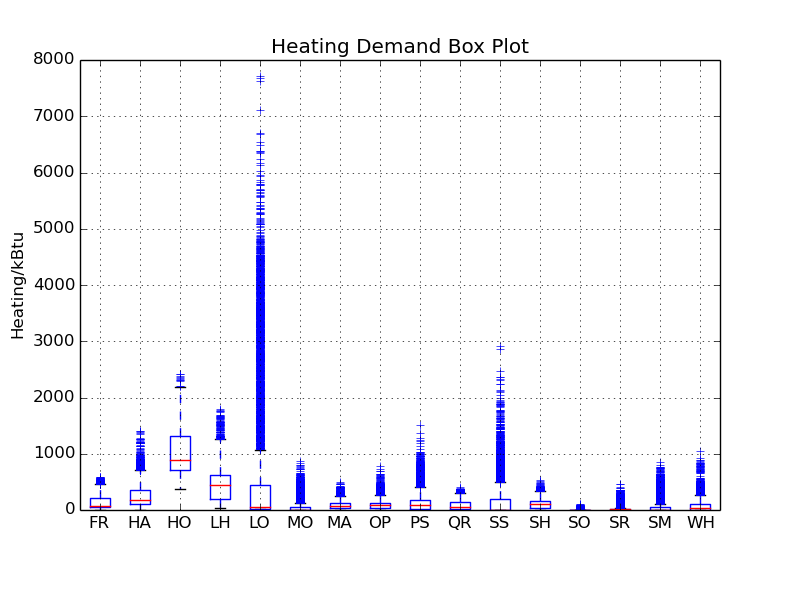
\includegraphics[width=\linewidth]{H}
  \caption[Heating Demand Box Plot]{Heating Demand Box
    Plot}
  \label{fig:H}
\end{subfigure}
~
\begin{subfigure}{0.4\textwidth}
  \centering
  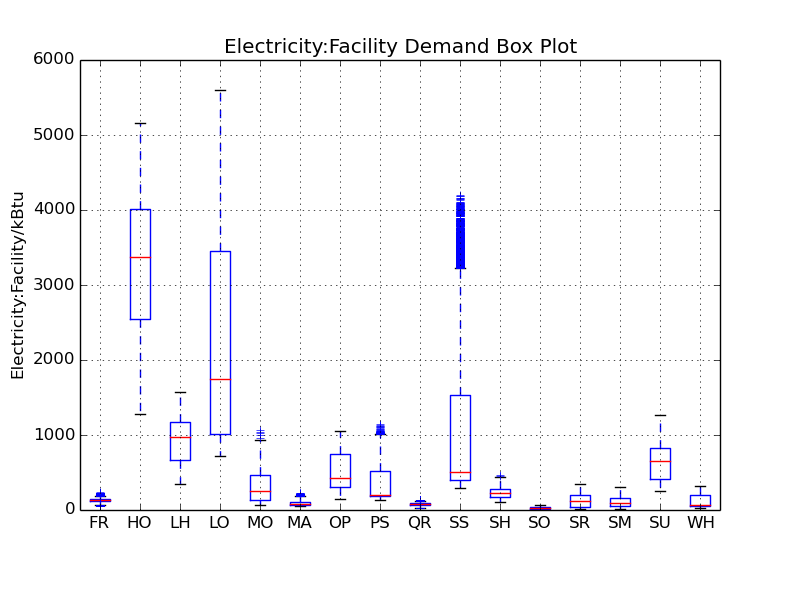
\includegraphics[width=\linewidth]{EF}
  \caption[Electricity Demand Box Plot]{Electricity Demand Box Plot}
  \label{fig:EF2}
\end{subfigure}
\caption[Comparing Heating and Electricity Demand]{Comparing Heating
  and Electricity Demand}
\end{figure}

\begin{figure}[h!]
  \centering
  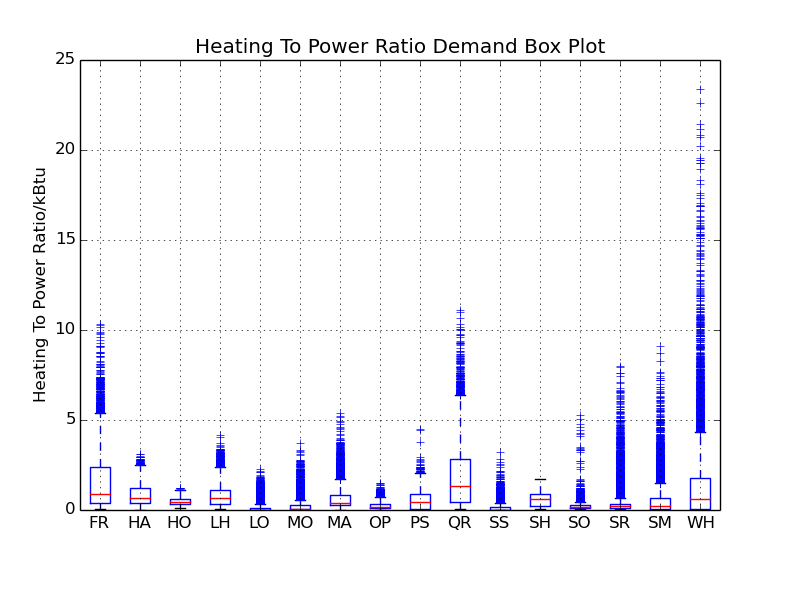
\includegraphics[width=0.7\linewidth]{HTPR}
  \caption[Heat to Power Ratio Box Plot]{Heat to Power Ratio Box Plot}
  \label{fig:HTPR}
\end{figure}%

\pagebreak
\subsubsection{Aggregated Demand Distribution}
This section analyzes the energy demand distribution of the hourly
energy demand (gas heating, electricity heating, service hot water,
cooling and electricity demand) of all buildings in the community. All
histogram show the distribution are very right skewed, so the researcher paired the
histogram of the original data with a histogram with natural log
scaling.

The difference in data distribution might influence the data
classification and energy data color-encoding, which then influences
the map display design. For example, as is explained in \sref{anime},
the continuous function from the energy demand to some color in a
color ramp seems to be more efficient in conveying the energy demand
changing pattern over time. In order to create such a mapping with
enough color or symbol variation, a transform function that reduces
the difference between the max and the min in the Probability Density
Function (PDF) of a distribution is important. Log scaling could be
one possible transformation function and is used in \sref{anime} for
the creation of the non-interactive gas heating demand animated map. A
closer look at how different energy data distribution can be better
visually inspected could be one of the topics for the next stage of
the project.

\begin{itemize}
\item Heating:

\begin{figure}[h!]
  \centering
  \begin{subfigure}{0.4\textwidth}
  \centering
  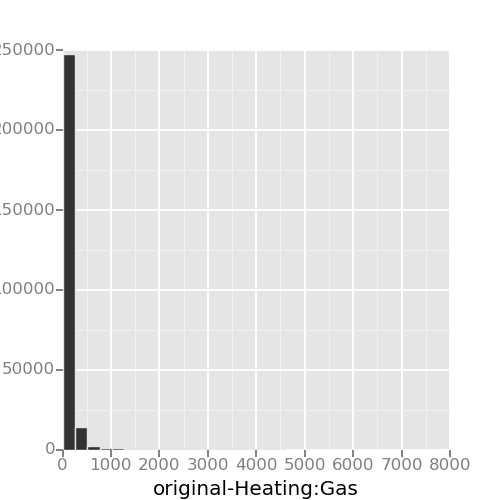
\includegraphics[width=\linewidth]{original-Heating:Gas}
  \caption[Gas Heating Demand]{Gas Heating Demand}
  \label{fig:original-Heating:Gas}
\end{subfigure}
~
\begin{subfigure}{0.4\textwidth}
  \centering
  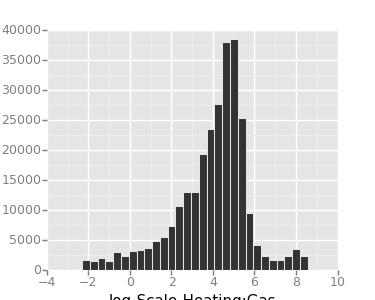
\includegraphics[width=\linewidth]{log-Scale-Heating:Gas}
  \caption[Gas Heating Demand]{Gas Heating Demand in Log Scale}
  \label{fig:log-Scale-Heating:Gas}
\end{subfigure}
  \caption[Gas Heating Demand Log]{Gas Heating Demand in Log Scale}
\end{figure}

\begin{figure}[h!]
  \centering
  \begin{subfigure}{0.4\textwidth}
  \centering
  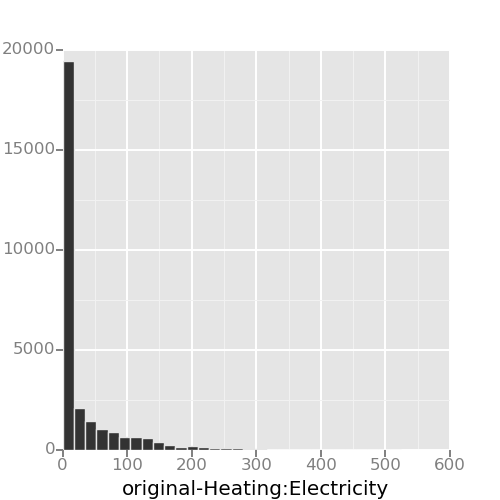
\includegraphics[width=\linewidth]{original-Heating:Electricity}
  \caption[Electricity Heating Demand]{Electricity Heating Demand}
  \label{fig:original-Heating:Electricity}
\end{subfigure}
~
\begin{subfigure}{0.4\textwidth}
  \centering
  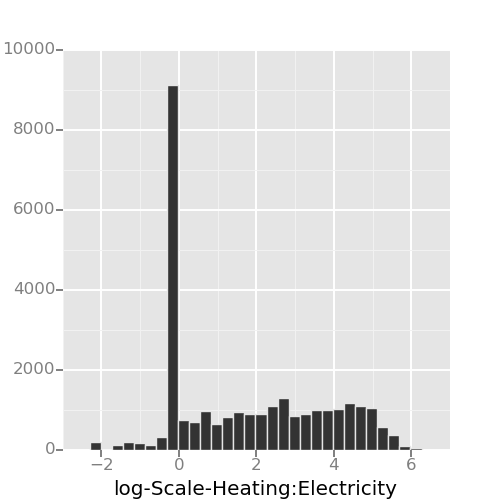
\includegraphics[width=\linewidth]{log-Scale-Heating:Electricity}
  \caption[Electricity Heating Demand]{Electricity Heating Demand in Log Scale}
  \label{fig:log-Scale-Heating:Electricity}
\end{subfigure}
  \caption[Electricity Heating Demand Log]{Electricity Heating Demand in Log Scale}
\end{figure}

\begin{figure}[h!]
  \centering
  \begin{subfigure}{0.4\textwidth}
  \centering
  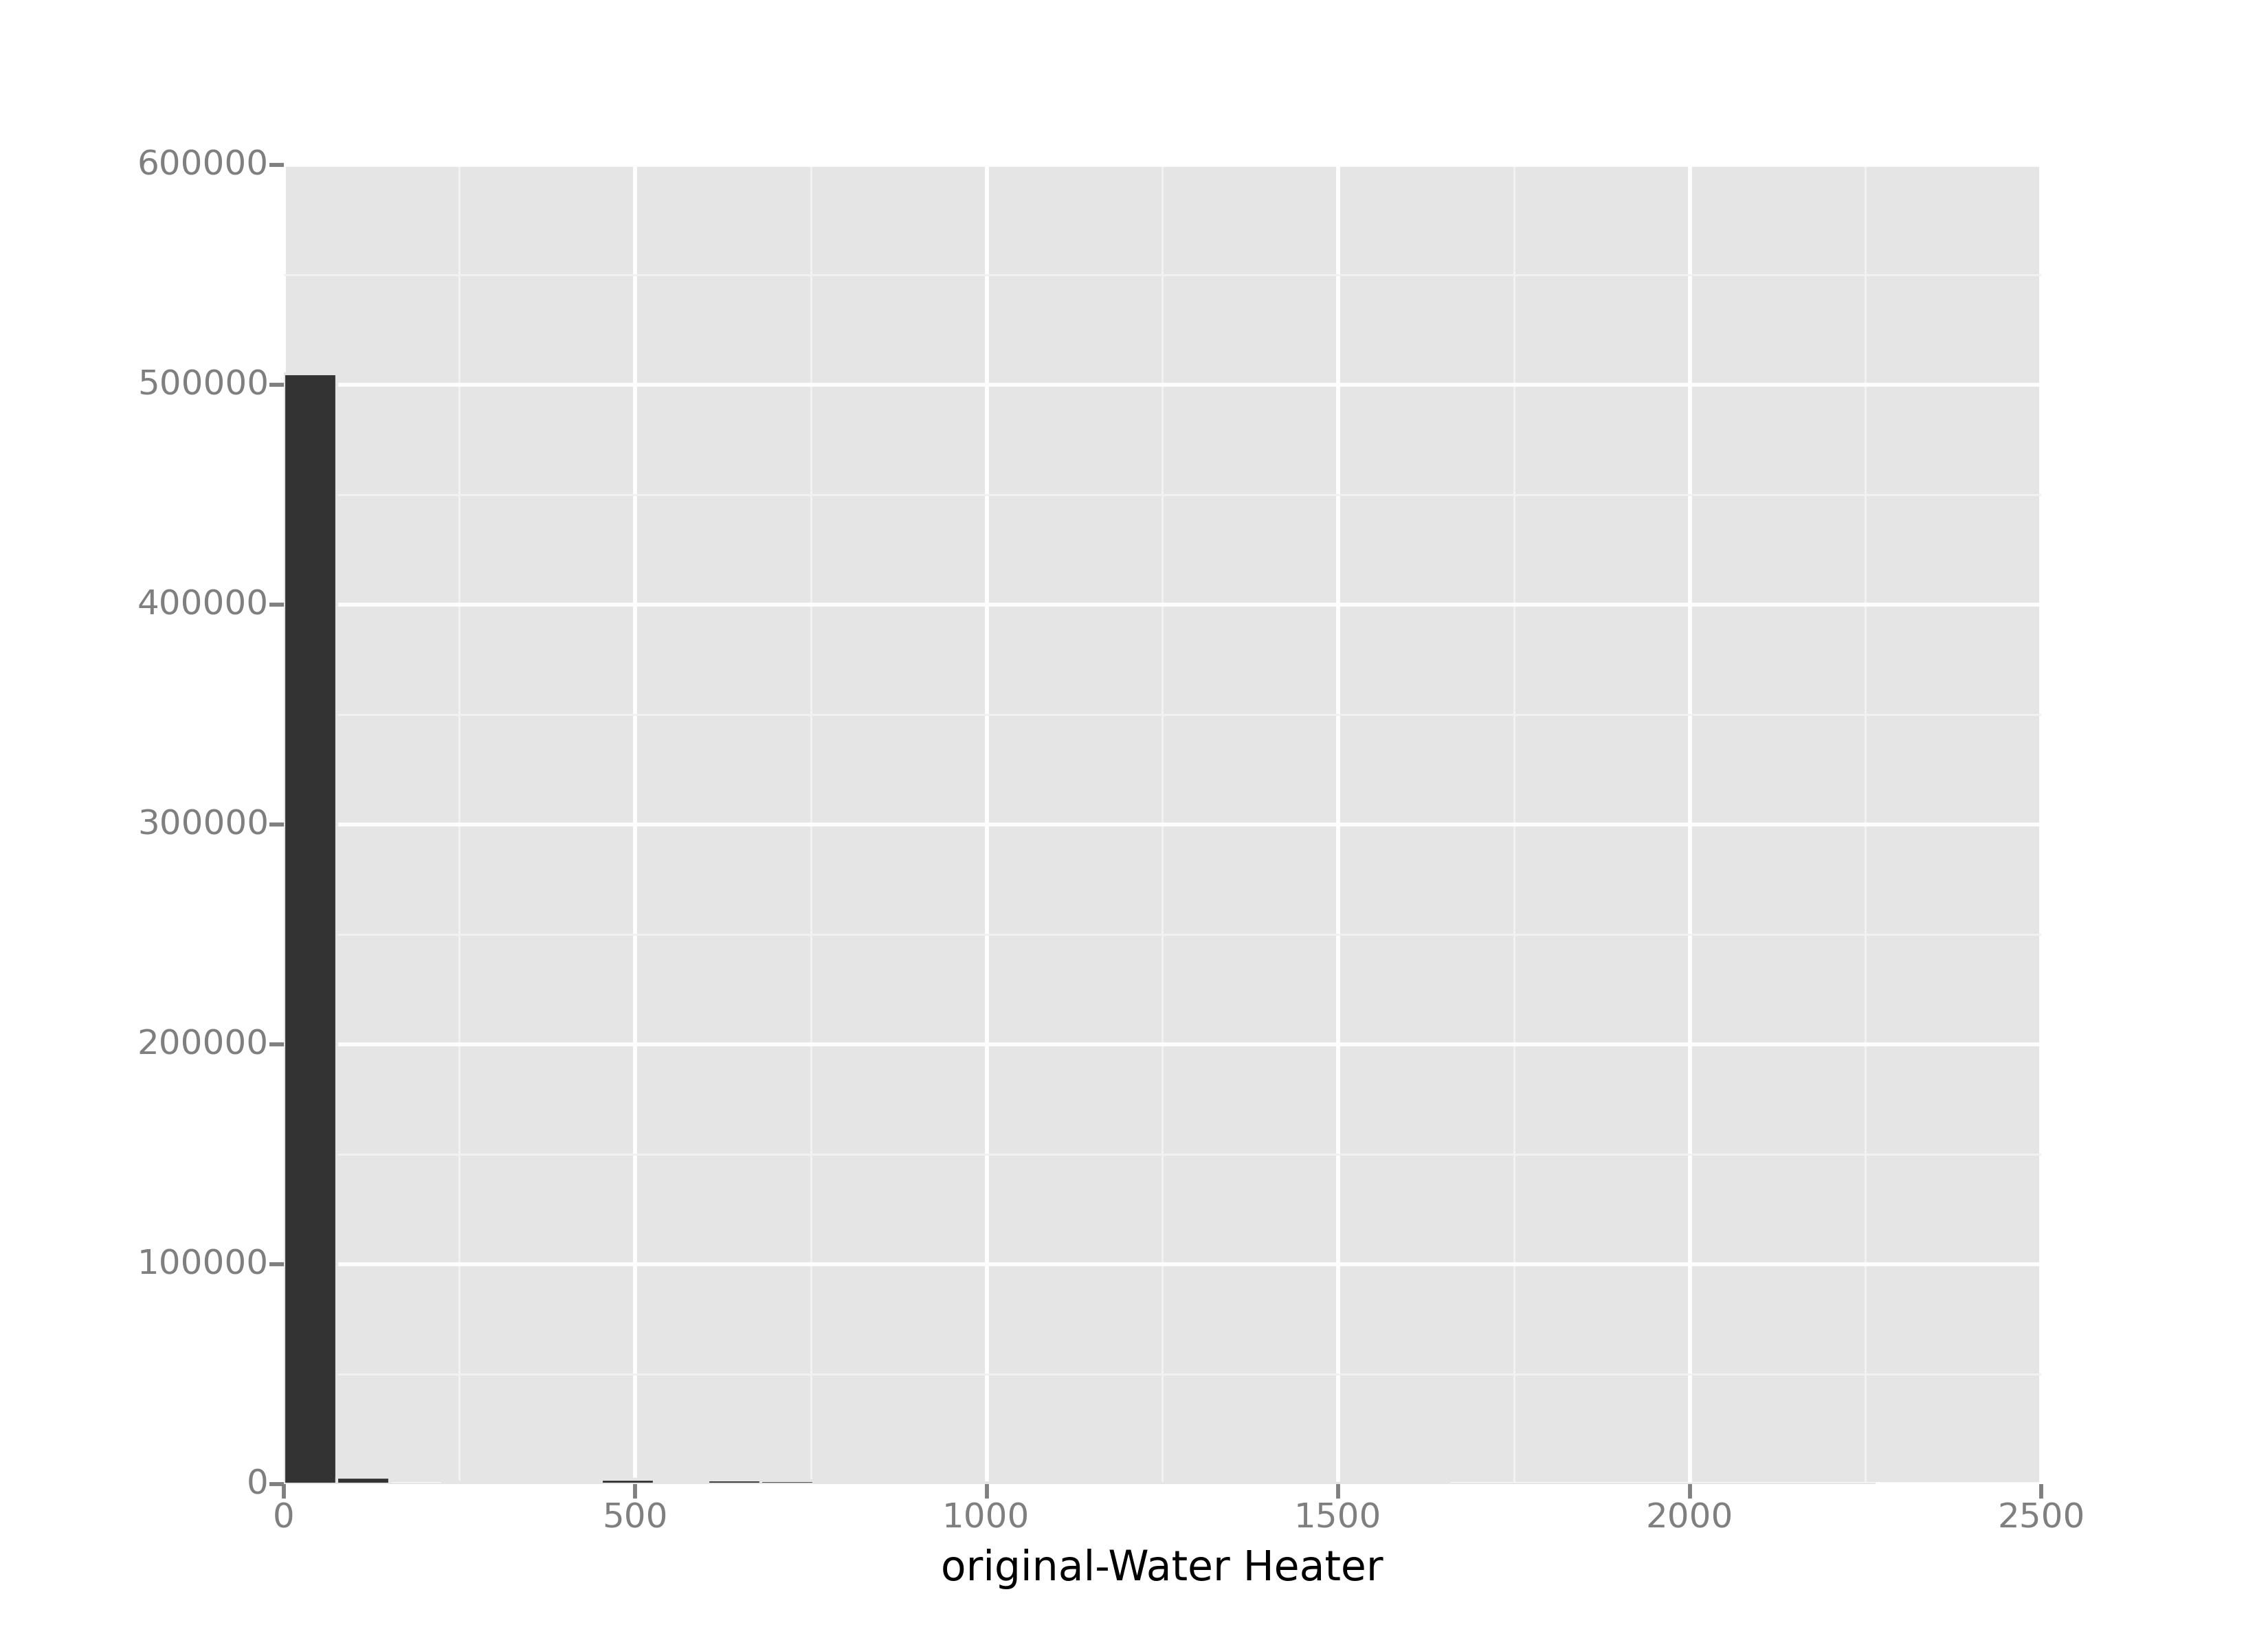
\includegraphics[width=\linewidth]{original-Water-Heater}
  \caption[Service Hot Water Demand]{Service Hot Water Demand}
  \label{fig:original-Water Heater}
\end{subfigure}
~
\begin{subfigure}{0.4\textwidth}
  \centering
  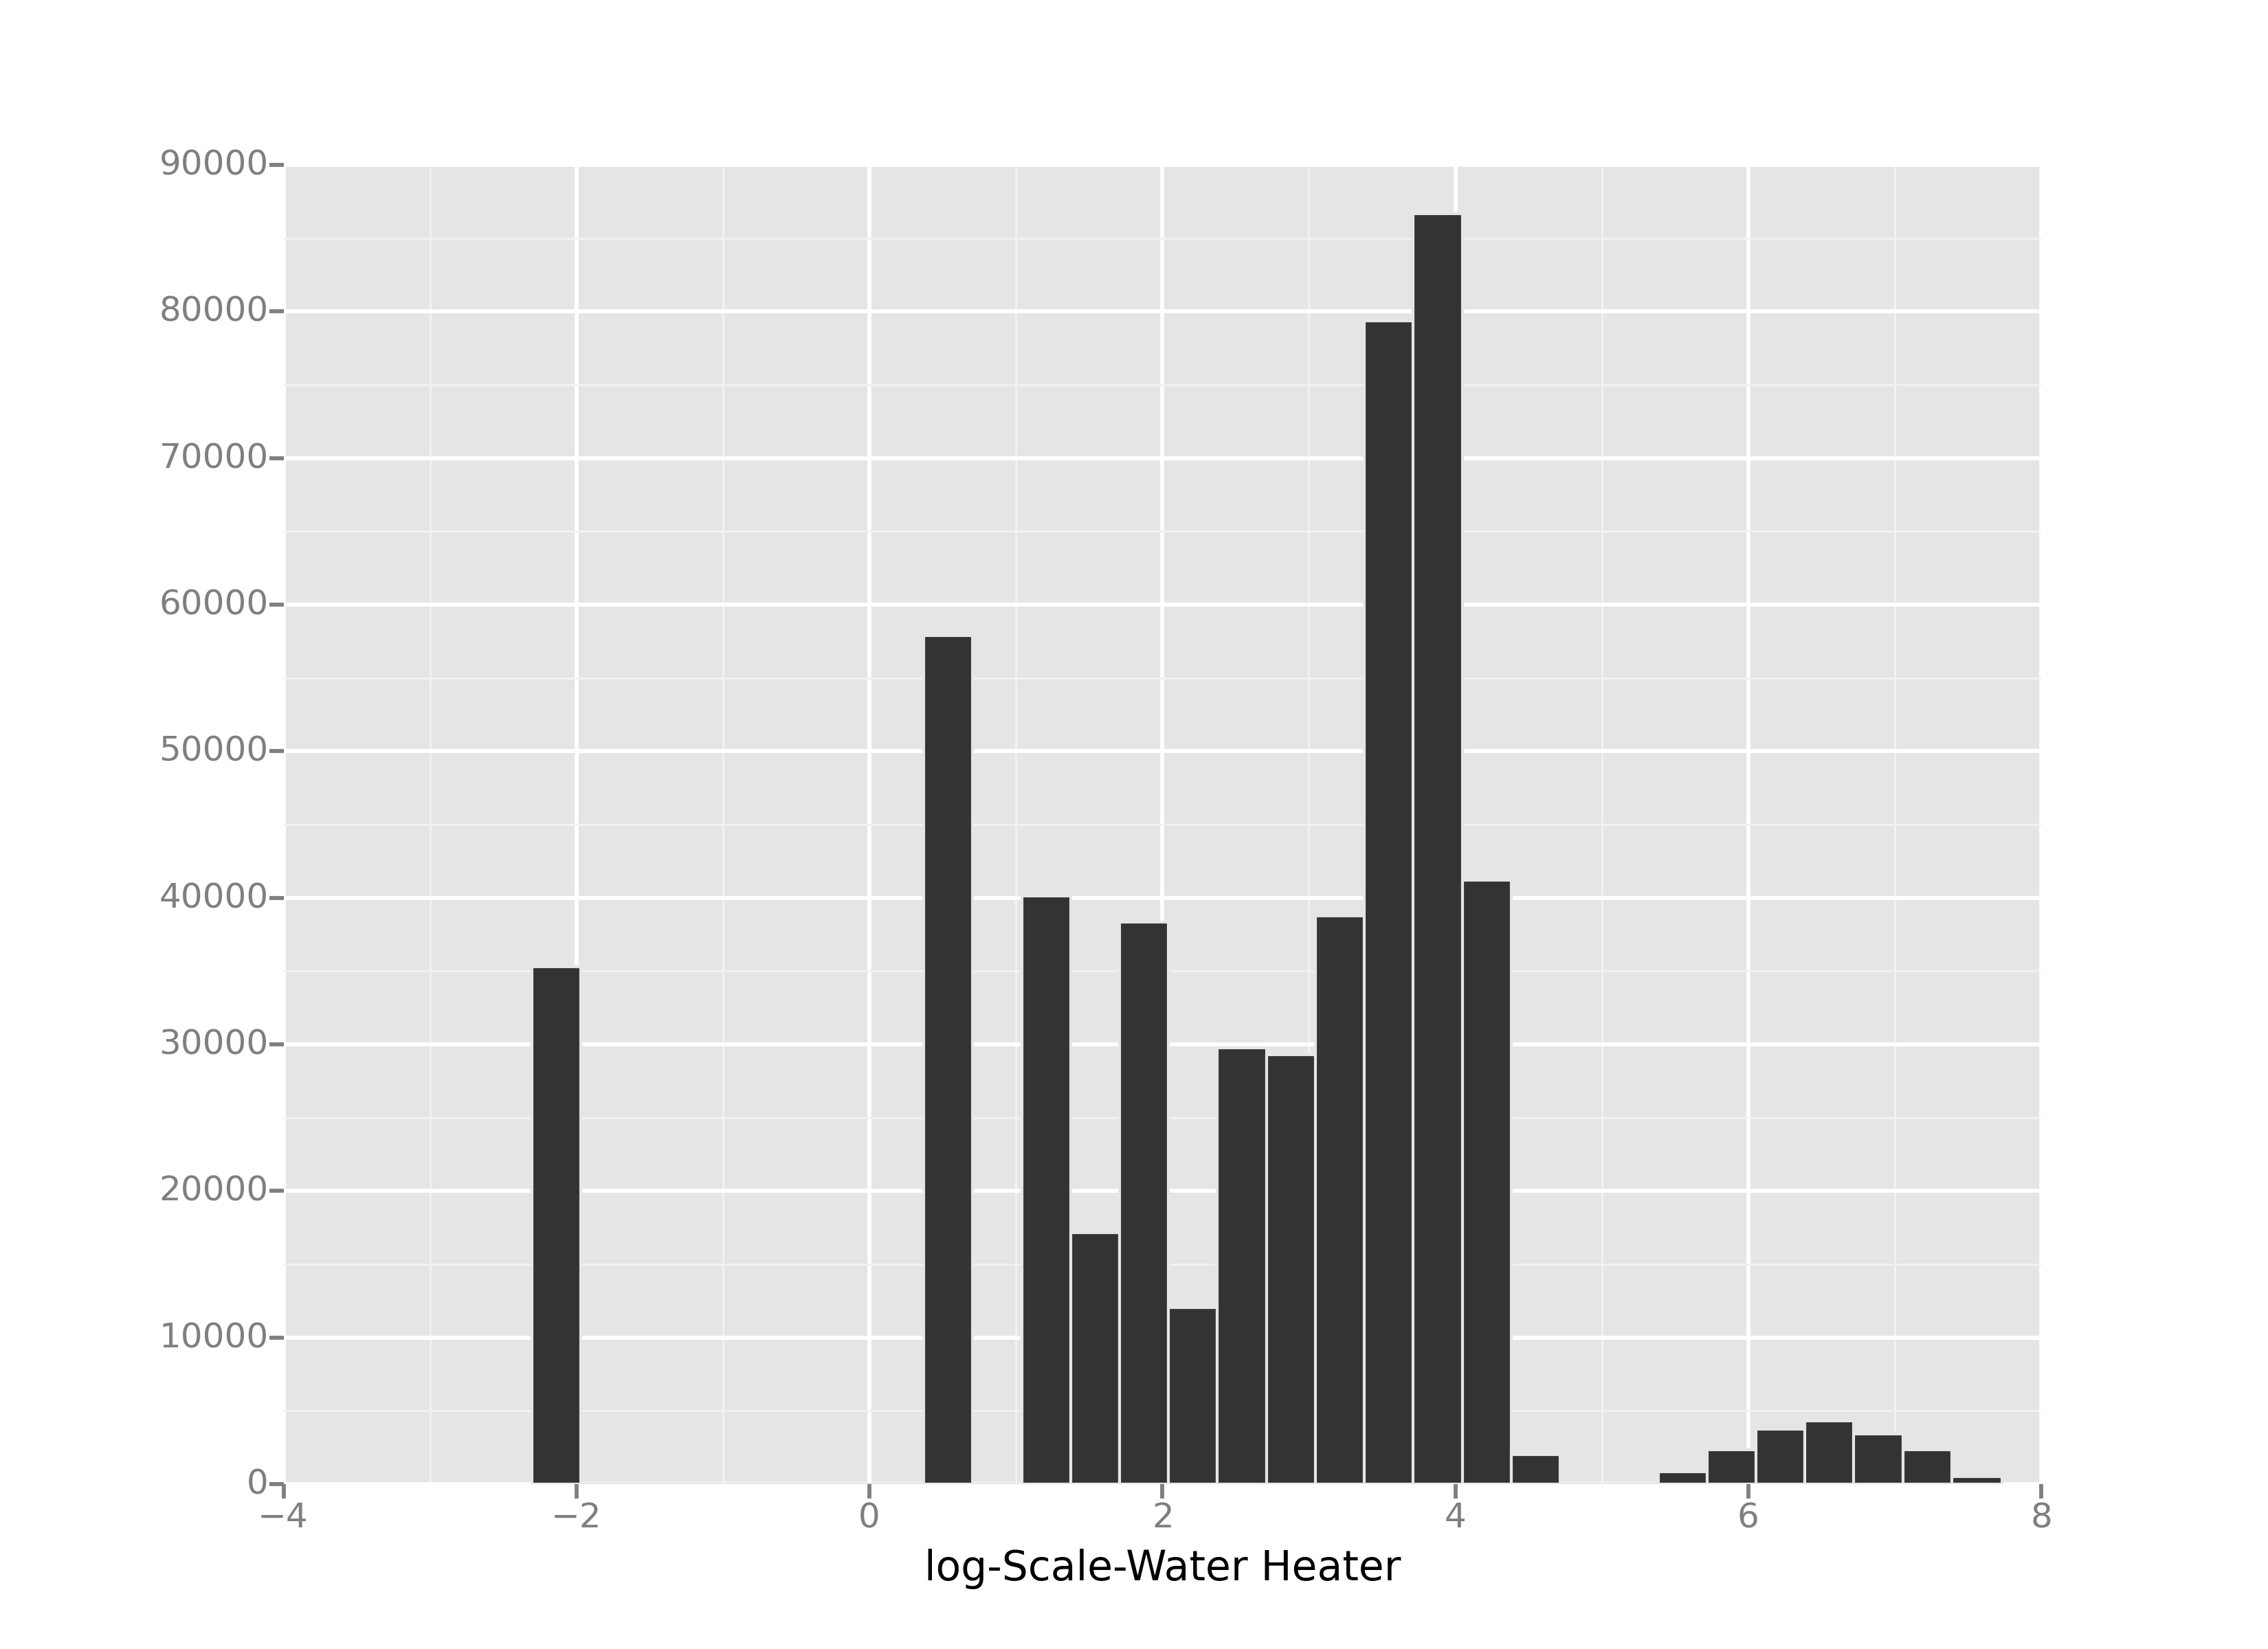
\includegraphics[width=\linewidth]{log-Scale-Water-Heater}
  \caption[Service Hot Water Demand]{Service Hot Water Demand in Log Scale}
  \label{fig:log-Scale-Water-Heater}
\end{subfigure}
  \caption[Service Hot Water Demand Log]{Service Hot Water Demand in Log Scale}
\end{figure}

\begin{figure}[h!]
  \centering
  \begin{subfigure}{0.4\textwidth}
  \centering
  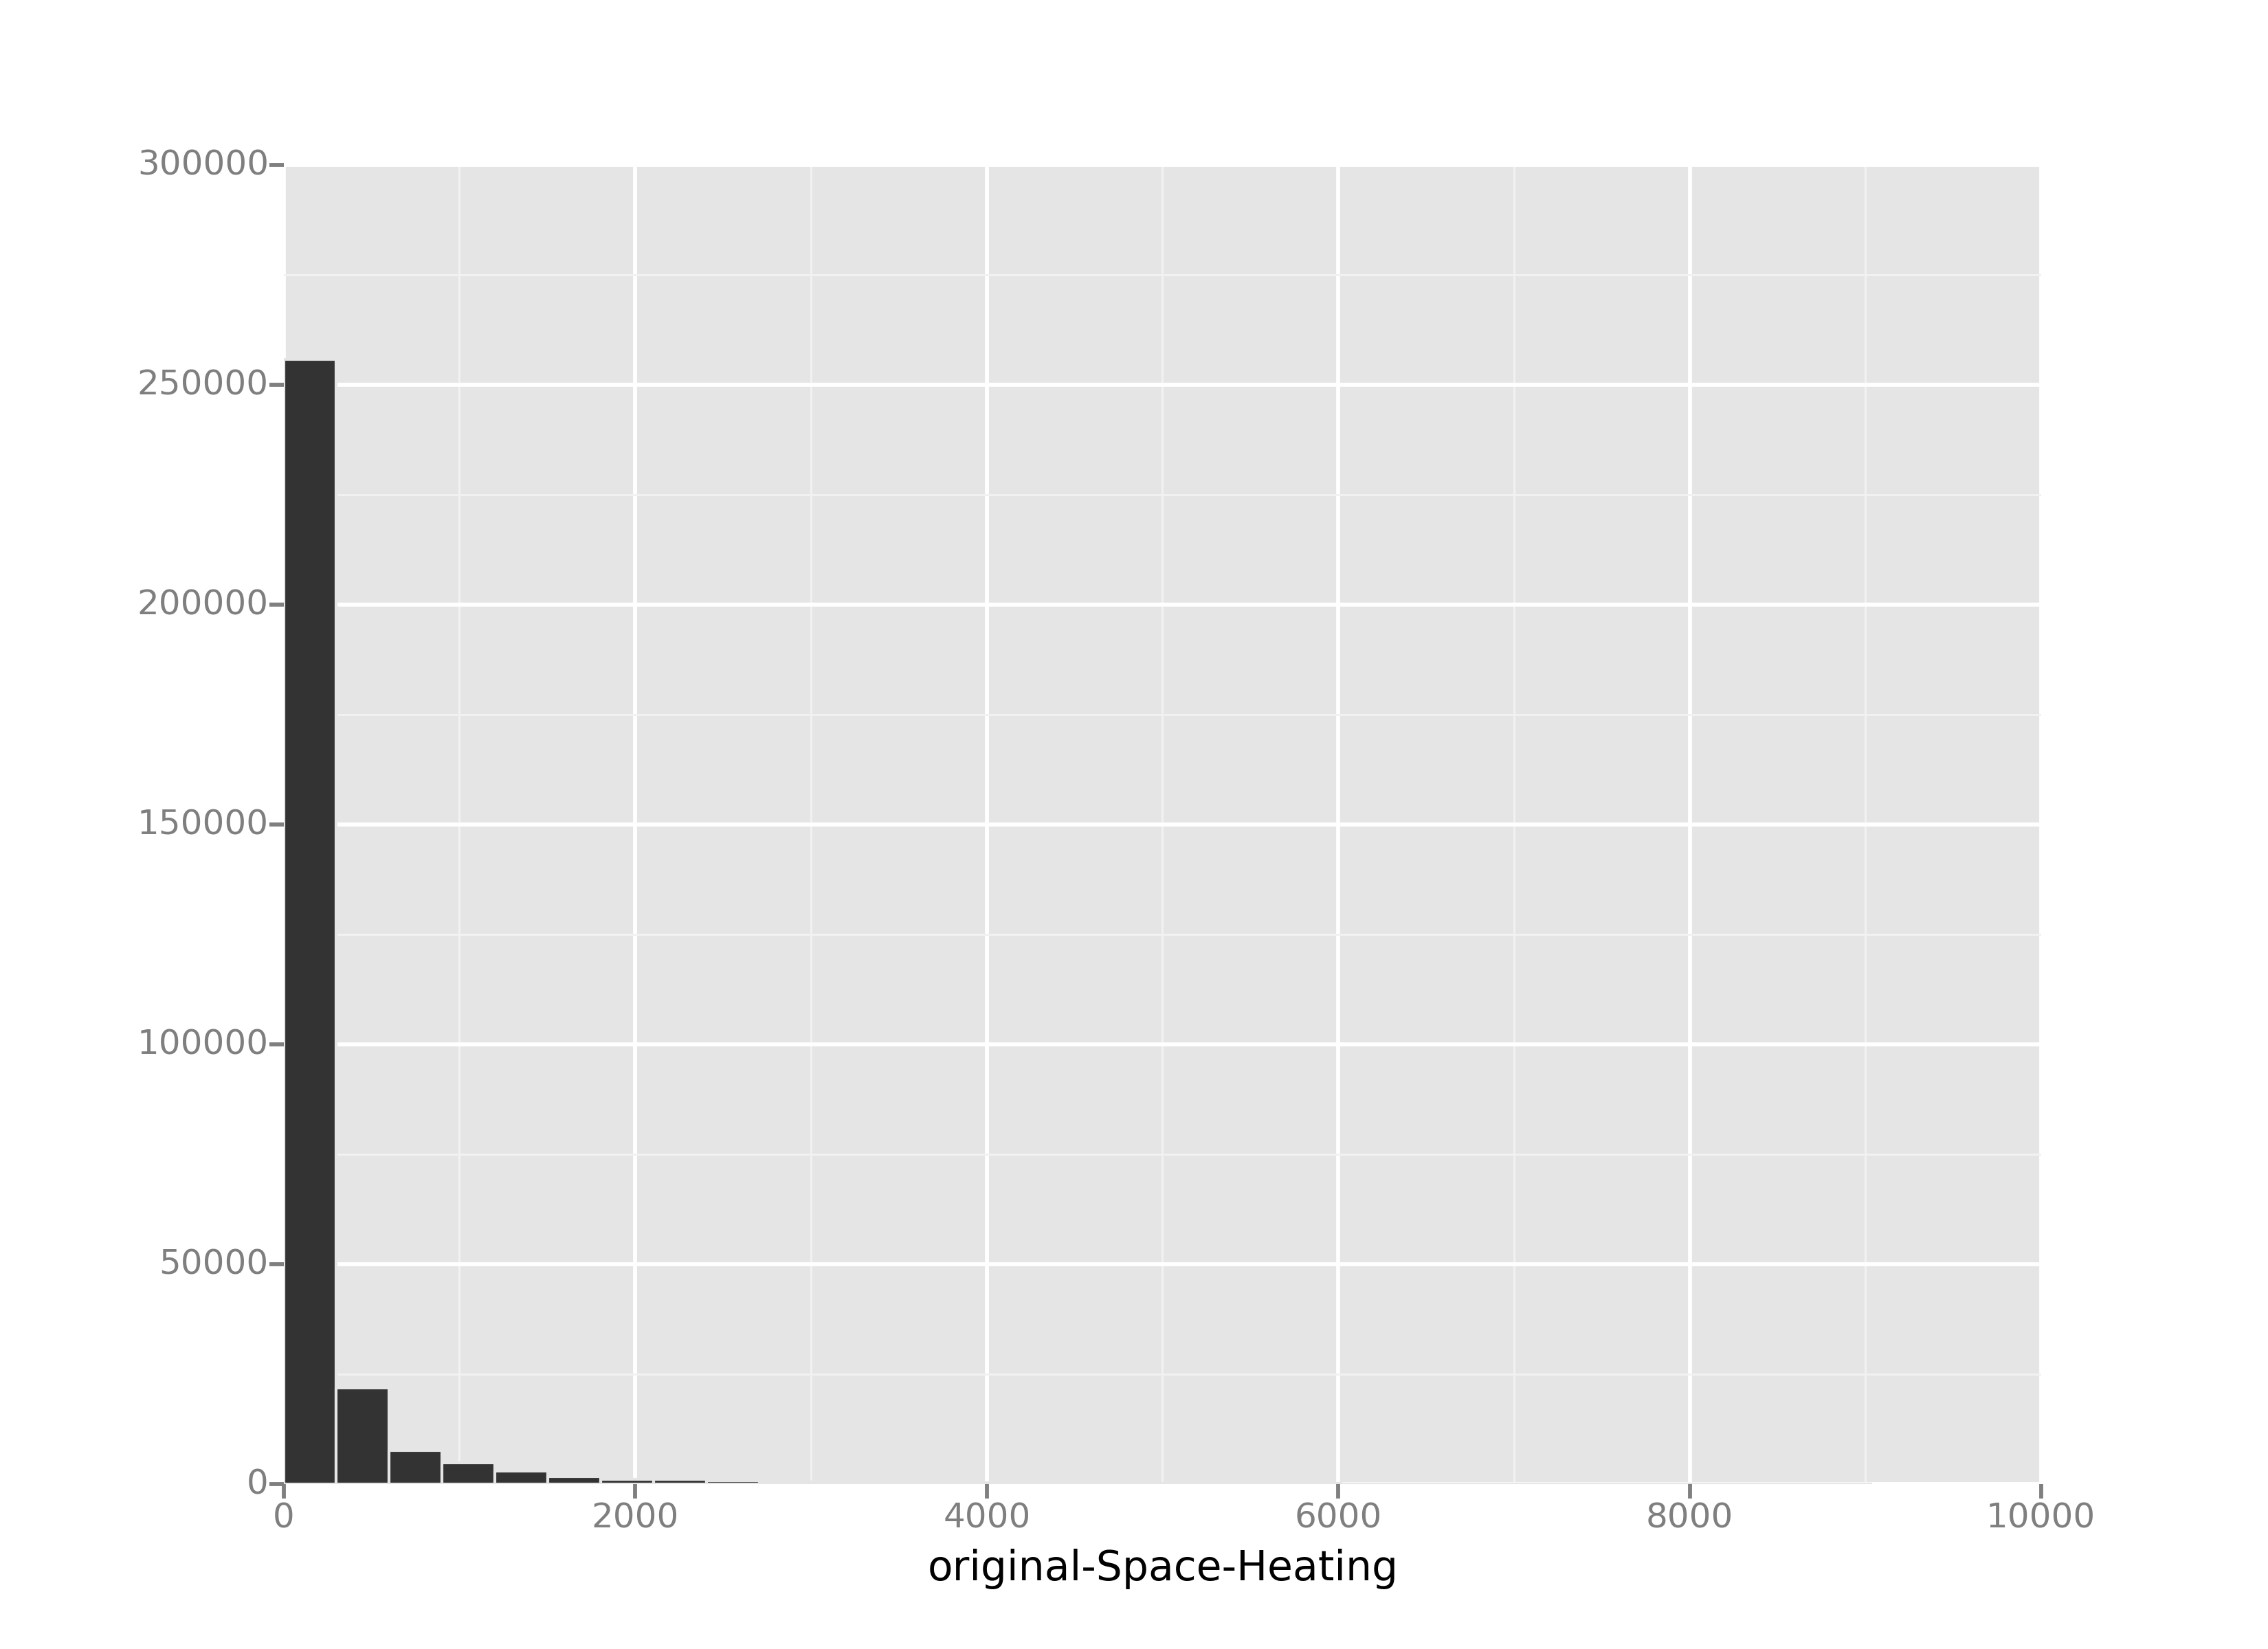
\includegraphics[width=\linewidth]{original-Space-Heating}
  \caption[Space Heating Demand]{Space Heating Demand}
  \label{fig:original-Space-Heating}
\end{subfigure}
~
\begin{subfigure}{0.4\textwidth}
  \centering
  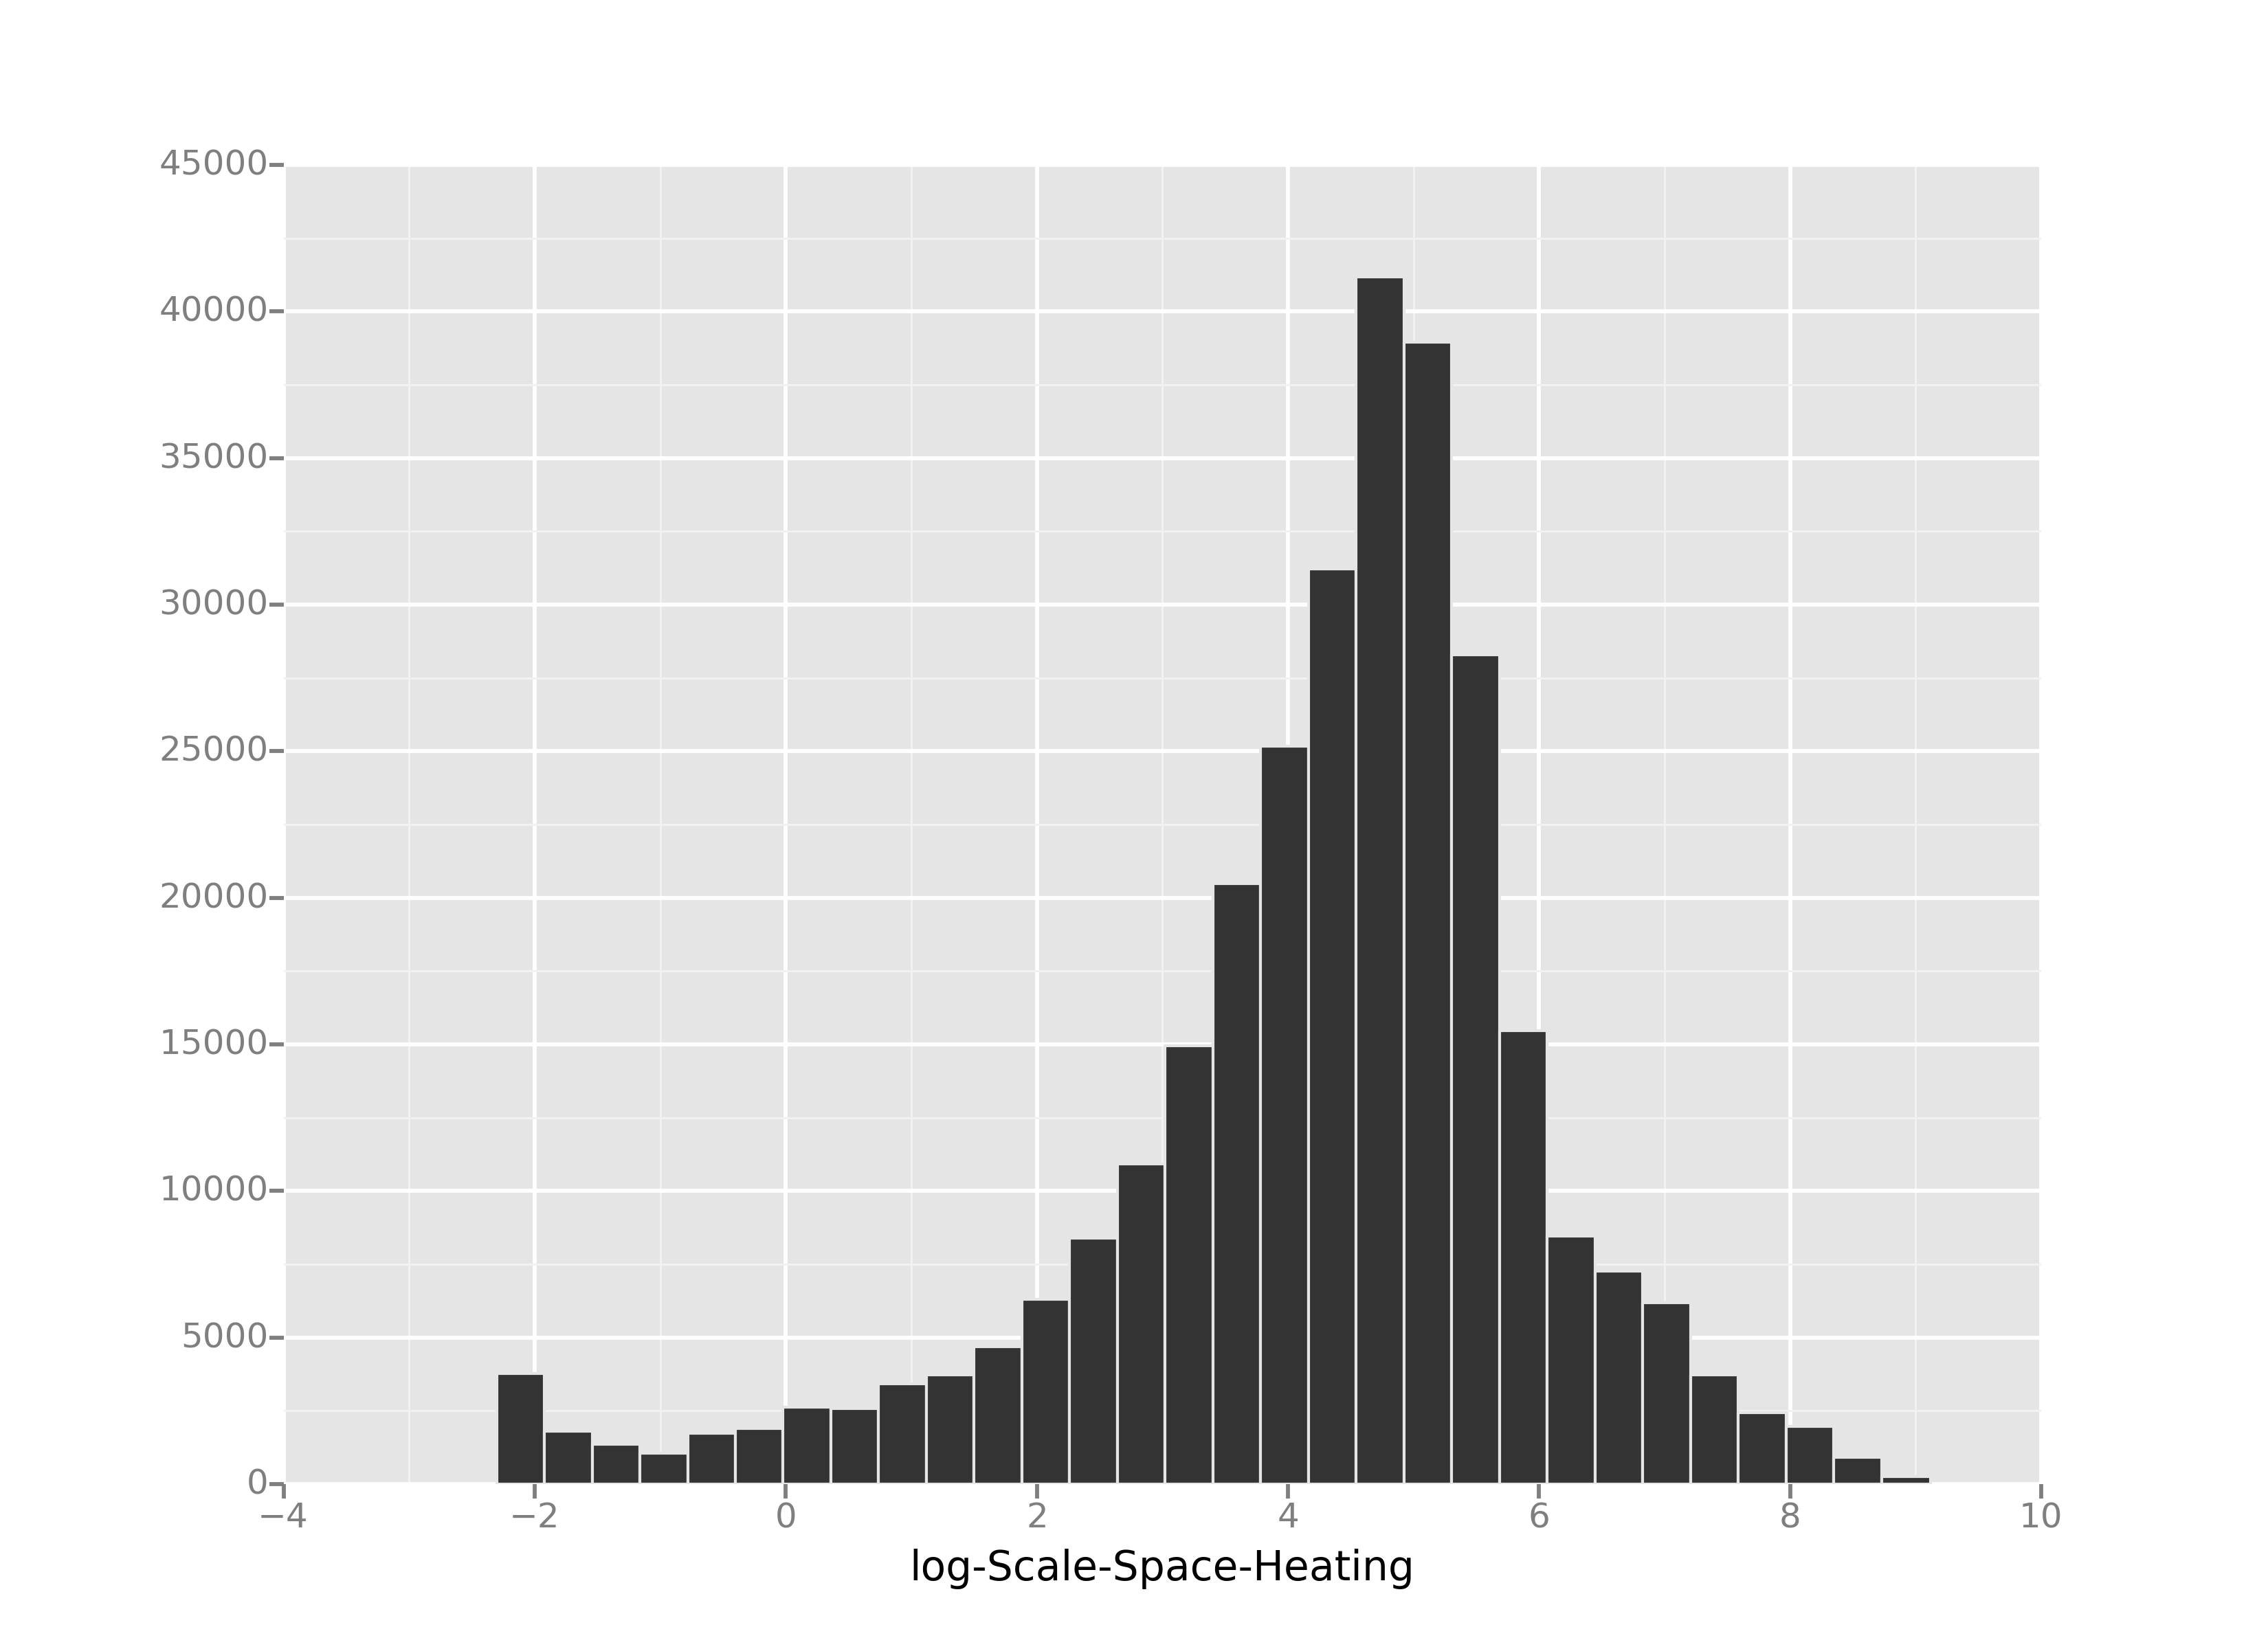
\includegraphics[width=\linewidth]{log-Scale-Space-Heating}
  \caption[Space Heating Demand]{Space Heating Demand in Log Scale}
  \label{fig:log-Scale-Space-Heating}
\end{subfigure}
  \caption[Space Heating Demand Log]{Space Heating Demand in Log Scale}
\end{figure}

\begin{figure}[h!]
  \centering
  \begin{subfigure}{0.4\textwidth}
  \centering
  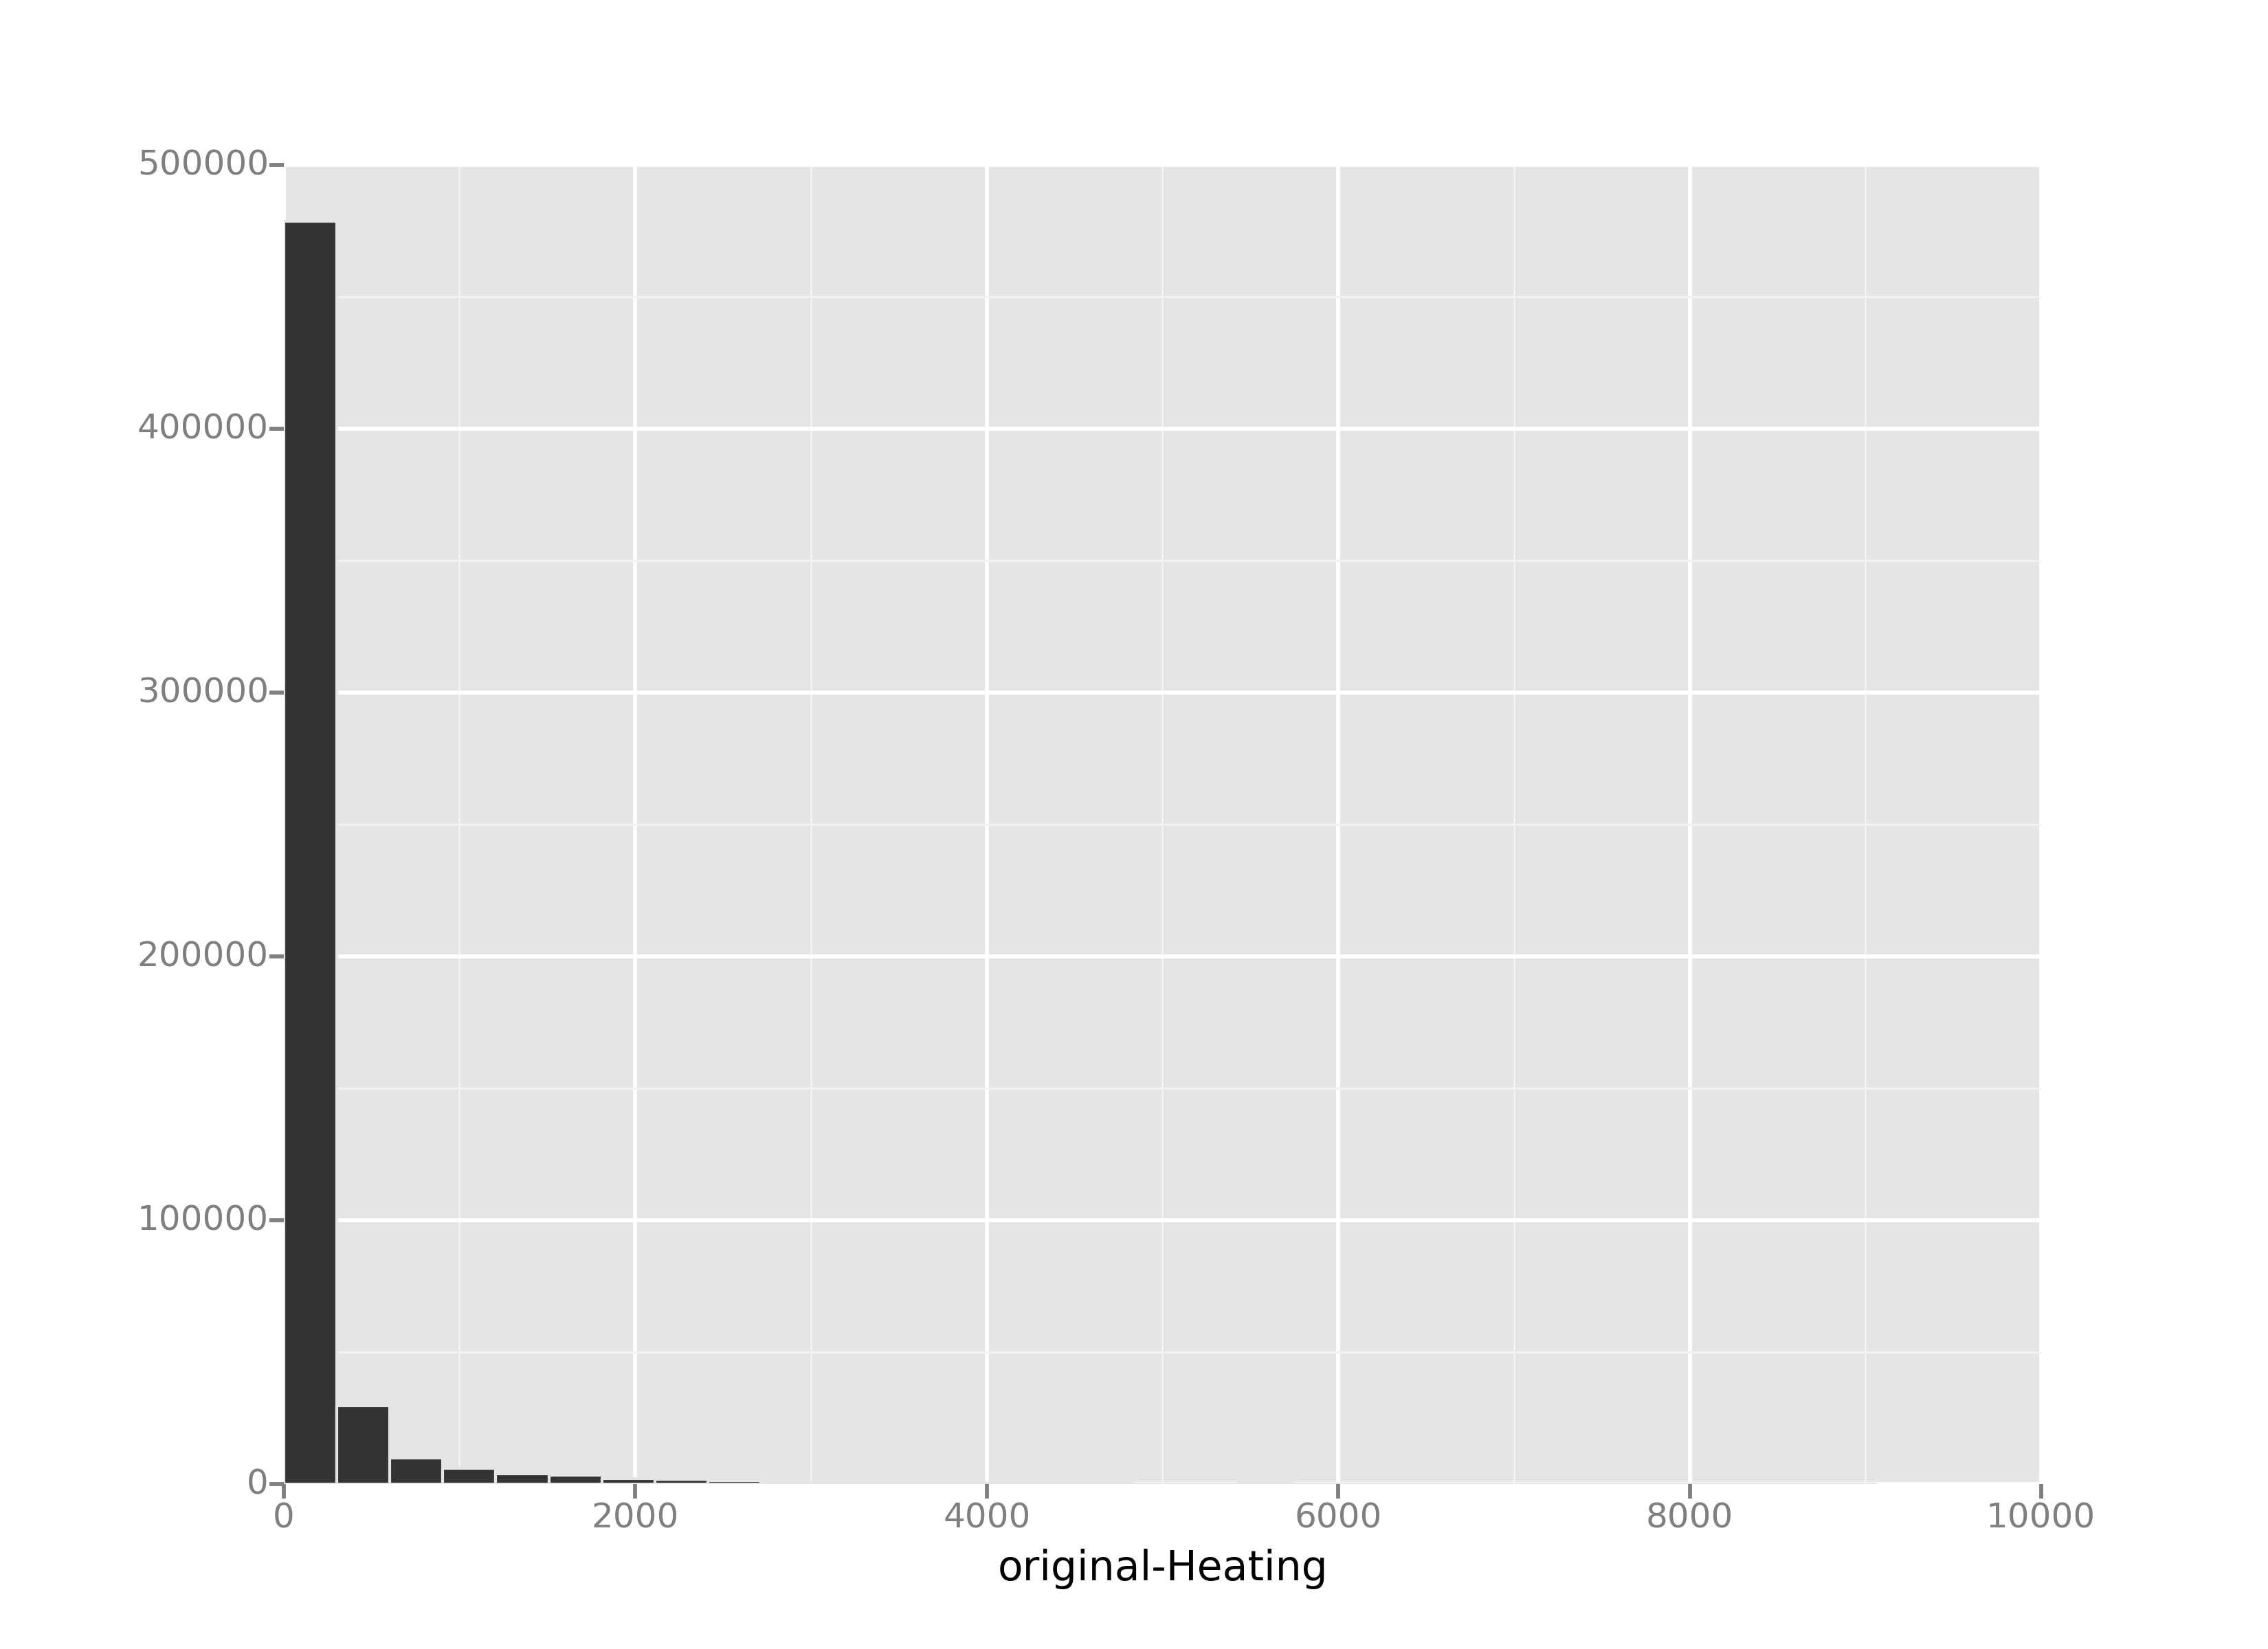
\includegraphics[width=\linewidth]{original-Heating}
  \caption[Heating Demand]{Heating Demand}
  \label{fig:original-Heating}
\end{subfigure}
~
\begin{subfigure}{0.4\textwidth}
  \centering
  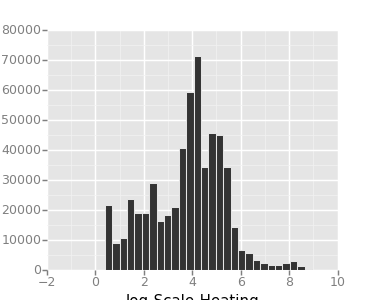
\includegraphics[width=\linewidth]{log-Scale-Heating}
  \caption[Heating Demand]{Heating Demand in Log Scale}
  \label{fig:log-Scale-Heating}
\end{subfigure}
  \caption[Heating Demand Log]{Heating Demand in Log Scale}
\end{figure}

\pagebreak
\item Cooling

\begin{figure}[h!]
  \centering
  \begin{subfigure}{0.4\textwidth}
  \centering
  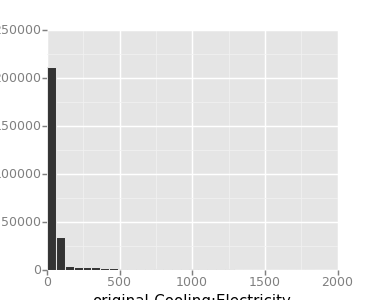
\includegraphics[width=\linewidth]{original-Cooling:Electricity}
  \caption[Electricity Cooling Demand]{Electricity Cooling Demand}
  \label{fig:original-Cooling:Electricity}
\end{subfigure}
~
\begin{subfigure}{0.4\textwidth}
  \centering
  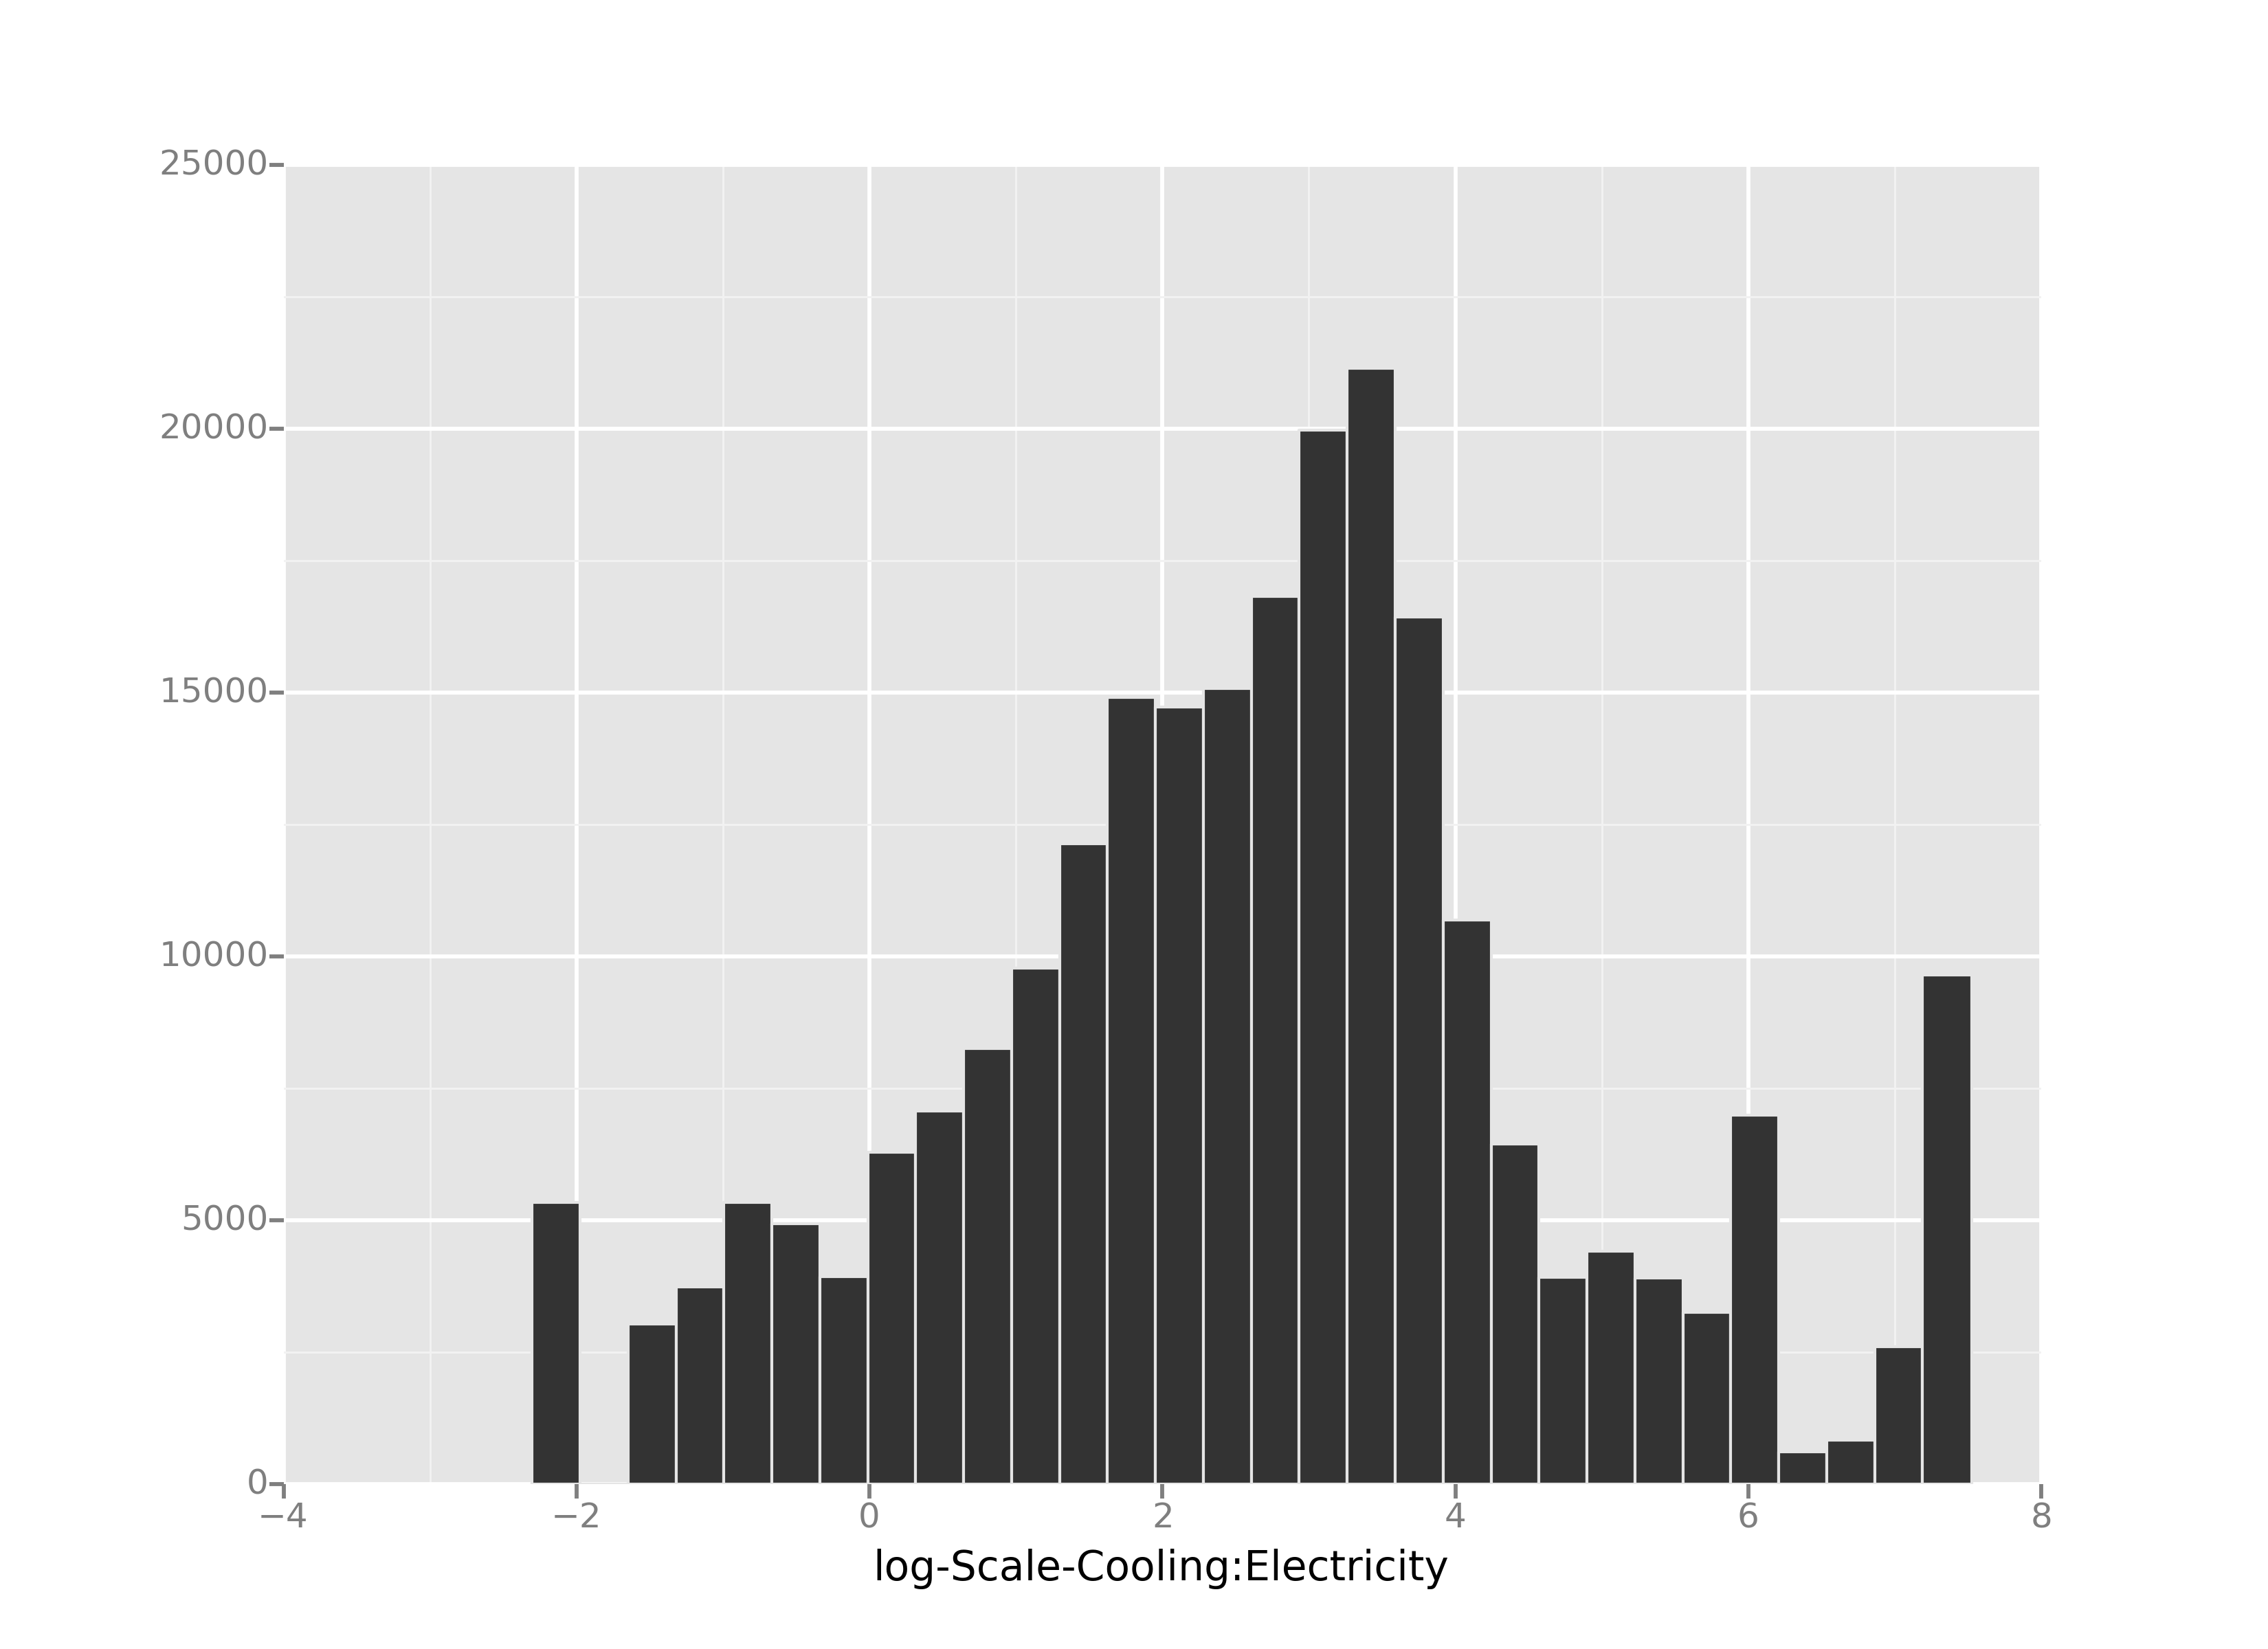
\includegraphics[width=\linewidth]{log-Scale-Cooling:Electricity}
  \caption[Electricity Cooling Demand]{Electricity Cooling Demand in Log Scale}
  \label{fig:log-Scale-Cooling:Electricity}
\end{subfigure}
  \caption[Electricity Cooling Demand Log]{Electricity Cooling Demand in Log Scale}
\end{figure}

\pagebreak
\item Electricity
\begin{figure}[h!]
  \centering
  \begin{subfigure}{0.4\textwidth}
  \centering
  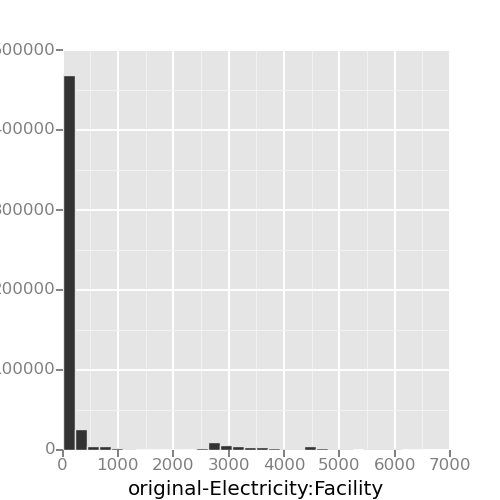
\includegraphics[width=\linewidth]{original-Electricity:Facility}
  \caption[Electricity  Demand]{Electricity Demand}
  \label{fig:original-Electricity:Facility}
\end{subfigure}
~
\begin{subfigure}{0.4\textwidth}
  \centering
  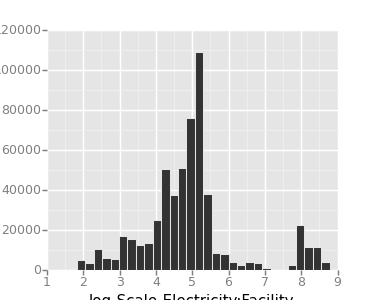
\includegraphics[width=\linewidth]{log-Scale-Electricity:Facility}
  \caption[Electricity  Demand]{Electricity  Demand in Log Scale}
  \label{fig:log-Scale-Electricity:Facility}
\end{subfigure}
  \caption[Electricity  Demand Log]{Electricity Demand in Log Scale}
\end{figure}

\end{itemize}
%%%%%%%%%%%%%%%%%%%%%%%%%%%%%%%%

\pagebreak
\subsection{3D GIS Model Geometry}
The conceptual community model is constructed in
CityEngine~\cite{cityEngine2015}. CityEngine is a software developed
by Esri~\cite{Esri2015}. It can aggregate geographic information into
buildings and is capable of smoothly transition models to
ArcGIS\cite{ArcGIS2015}, one of the widely applied tools for
Geo-referenced data presentation and analysis. Buildings in CityEngine
is defined with ``rules'' using CGA (Computer Generated Architecture)
shape grammar that is unique to CityEngine. The rule-based modeling of
urban environment enables fast construction and easy adjustability of
urban density, skyline and terrain control. It also enables easy
aggregation of Energy profile data into 3D urban environment models,
which is difficult to do in the current ArcGIS, the technical details
will be explained in \aref{AppendixA}.

Although the urban environment in this study is a conceptual setting,
I still want it to reflect the topological and density pattern in a
real urban environment. To construct the model, the researcher first extracted the
topological pattern from an existing urban design project, the Lower
Hill District Project~\cite{baird2014} (\fref{fig:mellonArena}.  There
are eight building types in the project: Residential (43\%), Town
House (2.9\%), Community Center (0.4\%), Commercial (3.8\%), Office
(19\%), Hotel (4.7\%), Cinema (1.4\%) and Garage (24.7\%).

\begin{figure}[h!]
  \centering
  \begin{subfigure}{0.5\textwidth}
  \centering
  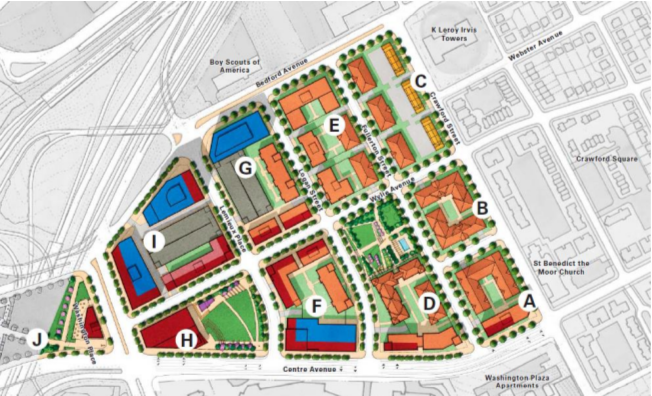
\includegraphics[width=\linewidth]{mellonArena}
  \caption[Lower Hill District Site Plan]{Lower Hill District Project Site Plan View}
  \label{fig:mellonArena}
\end{subfigure}
~
\begin{subfigure}{0.3\textwidth}
  \centering
  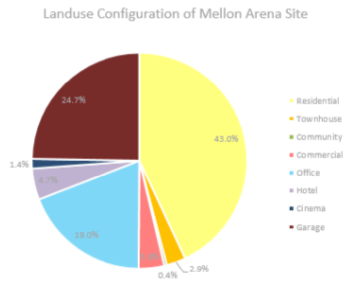
\includegraphics[width=\linewidth]{mellonPie}
  \caption[Lower Hill District Site Land Use]{Lower Hill District Site Land use Configuration}
  \label{fig:mellonPie}
\end{subfigure}
\end{figure}
The 16 building types in DOE commercial prototype models do not
perfectly correspond to those in the Lower Hill District Site. In order to
adapt the topological pattern of the Lower Hill District Project, a mapping
(function) from building types of Lower Hill District Site to building types
of DOE models is created as is shown in \tref{tab:typeMap}.
\begin{table}[h!]
  \centering
  \begin{tabular}{c| c| c}
    \hline
    Lower Hill District Type &Probability &DOE Building Type\\
    \hline
    \hline
    Hotel &50\%&Large Hotel\\
    \cline{2-3}
    &50\%&Small Hotel\\
    \hline
    Office &30\%&Large Office\\
    \cline{2-3}
    &30\%&Medium Office\\
    \cline{2-3}
    &30\%&Small Office\\
    \hline
    Residential &100\%&Midrise Appartment\\
    \cline{1-2}
    Townhouse &100\%&\\
    \hline
    Commercial &25\%&Full Service Restaurant\\
    \cline{2-3}
    $+$ Cinema $+$&25\%&Quick Service Restaurant\\
    \cline{2-3}
    Community &25\%&Strip Mall\\
    \cline{2-3}
    Center &25\%&Stand-alone Retail\\
    \hline
  \end{tabular}
  \caption{Mapping of Lower Hill District to Building Types of DOE prototype model}
  \label{tab:typeMap}
\end{table}

The four major building types involved in the current project are
residential, commercial, office and hotel. Their topological pattern
is represented in Figure \ref{fig:mellonTop}. The conceptual model
construction follows the building type topological pattern and the
urban density as the Lower Hill District Project (\fref{fig:sitePlan})

After the land use is assigned (\fref{fig:sitePlan}), one rule file is
applied to all the building lots and generates building geometries by
extruding the building lot (with an offset to the interior) according
to the number of floors of the prototype buildings. The building
geometry is simplified in order to highlight the color of each
building that encodes its energy demand.

\begin{figure}[h!]
  \centering
  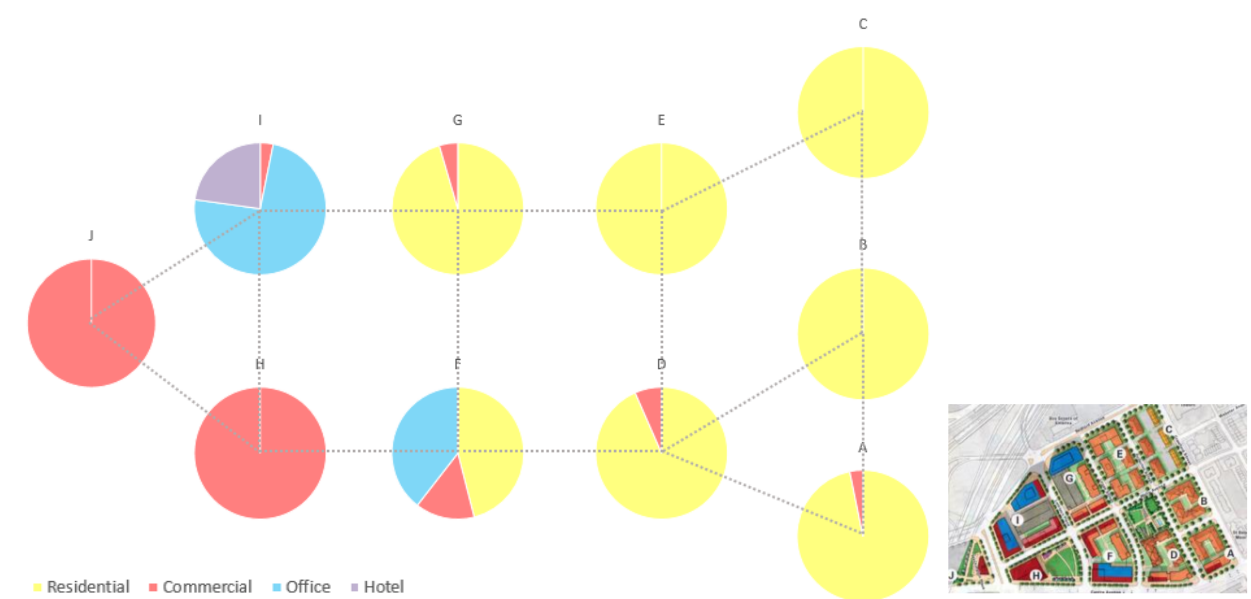
\includegraphics[width=\linewidth]{mellonTop}
  \caption[Building Type Topology]{Building Type Topological Pattern, Lower Hill District}
  \label{fig:mellonTop}
\end{figure}

\begin{figure}[h!]
  \centering
  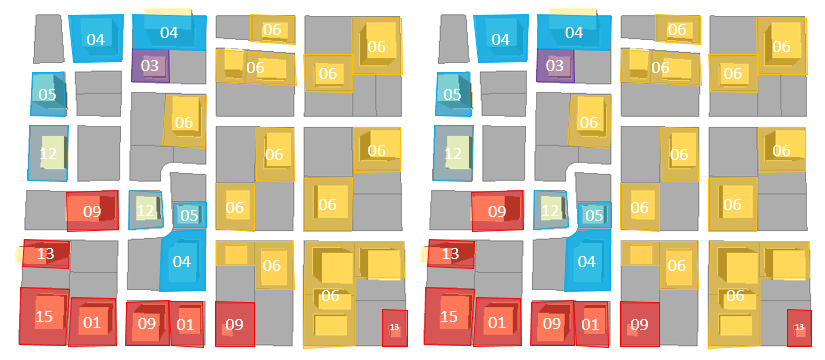
\includegraphics[width=\linewidth]{sitePlan}
  \caption[Conceptual Model Site Plan]{Site Plan of Conceptual Model}~ (01: Full Service
  Restaurant, 03: Large Hotel, 04: Large Office, 05: Medium Office,
  \\06: Midrise Apartment, 09: Quick Service Restaurant, 12: Small
  Office, \\13: Stand-alone Retail, 15: Strip Mall)
  \label{fig:sitePlan}
\end{figure}

%%%Book Mark
\subsection{Aggregating The hourly Energy Data to 3D GIS Model}\label{sec:aggregateTime}
\subsubsection{Comparing Different Approaches}
I have experimented with three approaches for aggregating energy
profile data into the conceptual model constructed in CityEngine were
tested.
\begin{enumerate}[1)]
\item Importing 3D models from CityEngine to ArcScene and aggregate
  the energy data (in the form of a table) into the 3D feature with
  ``one-to-many'' join. For more details please refer to
  \aref{AppendixC}

\item Write the energy profile data directly in the rule file for
  building generation in CityEngine. For more details please refer to
  \aref{AppendixA}

\item Process the color encoding outside of CityEngine and write the
  generated color encoding representations in CityEngine. This method
  allows for more specialized symbol and color map design.

\end{enumerate}

The first approach has the advantage of approach a ready-to-use data
classification method and map symbol templates that facilitates
choropleth map design and the ``time-slider'' function for creating a
time-wise navigation and animated map. \fref{fig:arcgisTime} shows the
interface slider and the dynamic map of heating energy demand for the
conceptual model using ArcGIS. 

There are several problems with this approach: 
\begin{itemize}
\item Its high requirement of computational power makes it infeasible
  to model or view on a typical PC.
  
  The researcher only succeeded in importing the hourly energy profile
  data when using point features to represent building geometry. Even
  for the relatively simple 3D models in the current study, with a
  relatively higher performance machine (Dell Precision T1600 Quad
  Core Intel Xeon, 3.10GHz RAM - 16GB was used) for importing the
  data, only one month of data could be imported. This technical issue
  makes it impossible to using the current ArcGIS platform to
  implement high temporal resolution dynamic maps without either
  truncating time range or reducing the complexity for building
  geometry representation.
\item The time dimension only exists inside the map file.

  This means even if one produced a dynamic energy map, one cannot
  share it without packing all related files and send to others. This
  requires the viewer to also have a high performance computer to view
  and manipulate the map. Although the animated map can be exported as
  an animation, the output animation contains neither any form of
  temporal label nor the control of playback. Without a time legend,
  the timing and duration of the dynamic changes are not shown.

\item For 3D GIS model, it does not contain a proper function to
  extract single frames of map images, making it impossible to create
  an exterior interface that deals with 3D maps images.

\end{itemize}

The second and third approach, on the contrary, provide more
flexibility but also requires much user-end work including:
pre-processing of energy profile data, implementing data
classification method and creating the bivariate color ramp. An
interface is also needed for visualizing the image sequence. Comparing
these two approaches that does not involve ArcGIS, since CityEngine
does not provide the bivariate color ramp, the color encoding cannot
be directly computed inside CityEngine, so the researcher chose the
method of processing the color encoding outside of CityEngine and
writing the generated color encoding representation into CityEngine
rule file for the final energy data aggregation method.

\begin{figure}[h!]
  \centering
  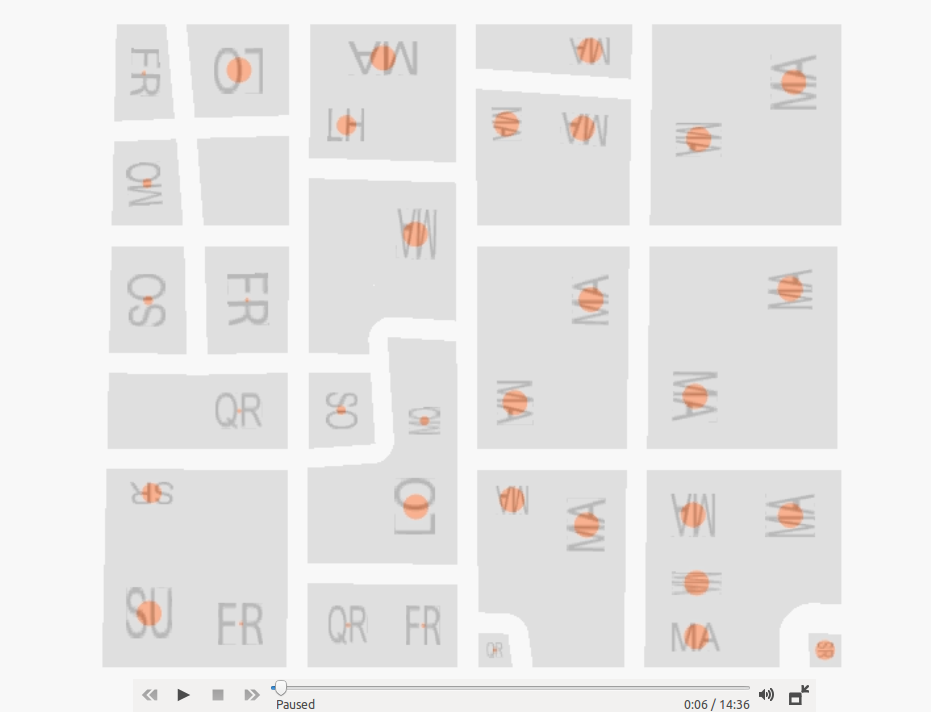
\includegraphics[width=0.5\linewidth]{arcgisTime}
  \caption{ArcGIS Time Slider for Temperal Data Display}
  \label{fig:arcgisTime}
\end{figure}

Due to limited time, the experimental GIS software uses only ArcGIS
and CityEngine. There might be better alternatives to achieve a
dynamic map with more elegance and also to put the stand-alone map
on-line to facilitate easy sharing. Finding a better alternative
software to implement a dynamic map could be part of the work of the
next stage of the project. Resch et al.\ evaluated some existing
web-3D and 4D visualization technologies~\cite{Resch2014} and found
WebGL to be competitive because of its high performance, portability,
spatial coordination support with three.js framework and no
requirement of plug-in etc ~\cite{Resch2014}.

\subsubsection{Data Classification}\label{dataClassification}
This researcher developed a function to translate energy data to its
color representation in order to visualize energy data in the map. A
common approach is to create a series of graduated colors or symbols
and to classify the data into a few groups, assign each group one
color or symbol in the series of symbols.

In order to write the data classification routine for the
demonstration of dynamic energy map in the current study, the
researcher conducted a brief survey of the commonly used GIS software
for commonly applied data classification methods. The software
surveyed in the study include: ArcGIS~\cite{GIS_Jenks2014}, GRASS
GIS~\cite{GRASSGIS2008}, gvGIS~\cite{gvGIS2011}, and QGIS. The data
classification method adopted by the surveyed software in creating a
thematic map include: 1) equal interval, 2) quantile 3) Jenks 4)
Standard Deviation 5) pretty breaks and 6) manual interval (use
context specific break point values). The common data classification
method shared by all surveyed instances are ``Equal Interval'',
``Quantile'' and ``User Defined''. Therefore the researcher chose to
implement the ``Equal Interval'' and ``Quantile'' method were selected
for the current project.

\begin{table}[h!]
  \centering
  \begin{tabular}{r|c c c c c c}
    \hline
           & Equal Interval & Quantile & Jenks & Pretty Breaks & StDev & User Defined\\
    \hline
    ArcGIS &      o        &    o     &  o    & x &  o  &   o  \\
 GRASS GIS &      o        &    o     &  x    & x &  o  &   o  \\
     GVSIG &      o        &    o     &  o    & x &  x  &   o  \\
      QGIS &      o        &    o     &  o    & o &  o  &   o  \\
    \hline
  \end{tabular}
  \caption{Data Classification Method (o: yes, x: no)}
  \label{tab:classify}
\end{table}

From the distribution of energy data in \cref{Chapter4}, a severe
right skew was observed in energy data distribution of single
buildings and the community. If using the ``Equal Interval'' method,
the display will lack variation between different frames because the
majority of data points will be concentrated in the low-energy demand
end. For example, in the distribution shown in
\fref{fig:original-Heating:Gas}, over 84\% of the data points are
between 0 to 1000. If using equal interval with 8 classes, all 84\% of
the data will be classified into the first group. This means the
difference in the majority of the energy demand between buildings are
not effectively shown. For ``User Defined'' breakpoints, further study
or survey will be necessary to decide the set of robust breakpoints
based on specific building energy context. The ``Quantile'' method is
thus chosen as the data classification method for the demonstration of
the functions of the dynamic energy map interface
(\fref{fig:legend2d}). This method makes sure every class has the same
number of points in it which ensures a balanced color display in each
frame of the dynamic energy map. Since the heating and cooling demand
are seasonal for most building types, there are a great portion (50\%)
of hours in a year with zero heating or cooling demand. If calculated
directly, the ``Quantile'' method will output several classes with
their members all being zero, leading to the effect of representing
the same value zero with different colors or symbols. Thus zero is
eliminated in calculation of break points.

The color for every building type in every hour of the year is
computed with a Python program from the input energy demand data of
heating, cooling and electricity. The output of the program is a text
file that could be directly copied into CityEngine.

\section{Output Map Images}
After the energy information was aggregated into the CityEngine model,
map images are could be generated. The map images are extracted as
snapshots from CityEngine with Python script by iterative setting the
time step and extracting a snapshot of that time step:

\makeatletter
\def\verbatim@font{\linespread{1}\tiny\ttfamily} \makeatother
\begin{verbatim}
'''
Created on Jun 5, 2015
@author: yujie
'''
from scripting import *
import time

# get a CityEngine instance
ce = CE()

def main():
    x = ce.getObjectsFrom(ce.scene, ce.withName("'LOT'"))  # < 1s
    for i in range(2):
        for item in x:
            ce.setAttribute(item, 'time', i) # 28 s
            views = ce.getObjectsFrom(ce.get3DViews())  # < 1s
        if i < 10:
            views[0].snapshot(ce.toFSPath('images')+("/img000"+str(i)+".png"))
        elif i < 100:
            views[0].snapshot(ce.toFSPath('images')+("/img00"+str(i)+".png"))
        elif i < 1000:
            views[0].snapshot(ce.toFSPath('images')+("/img0"+str(i)+".png"))
        else:
            views[0].snapshot(ce.toFSPath('images')+("/img"+str(i)+".png"))

if __name__ == '__main__':
    main()
\end{verbatim}
After this step, a sequence of 8760 3D (if using perspective view) or
2D (if using top view) energy images were extracted and named
according to their time stamp (``imgxxxx.png'' represents the energy
demand for the xxxx-th hour)

\section{Interface Specification}\label{interfaceSpec}
As is addressed in \sref{sec:aggregateTime}, an interface is needed to
combine the map image sequence with data plot and to provide the
ability to visualize and analyze more complicated spatial-temporal
data. In this section the researcher provides some abstract
specification of the functions of the interface are offered, in
\cref{Chapter6} a more detailed illustration of the design and
application of the interface is given.

\subsection{User Definition}
First the researcher want to specify a user profile in order to best
convey the information with the Dynamic Energy Map.

The potential category of user group for the Dynamic Map includes: 1)
policy makers, 2) urban planners with the interest in executing
community level energy strategies 3) researchers in energy related
fields 4) public groups or individuals that are involved or interested
in the decision making process of community energy planning.

The target user for the current interface design is restricted to
researchers in energy related fields. The assumption about this user
group about their skill level and background knowledge is that 1) they
have the basic ability to read and understand the layout of a map
environment and can associate it with the urban environment setting
they are associated with 2) they have the ability to correctly
understand moderately complicated map legend and data plot 3) they
have a basic understanding of building energy performance attributes
and the general implications of these attributes. The assumptions
about their intention is that they might have different research
interest and focus. These assumptions implies the interface design
should: 1) provide both qualitative and quantitative information; 2)
allow for some degree of user control over data classification, legend
selection and full control over time navigation. 

\subsection{Function Specification}
The major function of the interface is in general defined as:
``\textbf{Revealing the spatial-temporal heating, cooling and
  electricity demand variation of the conceptual model with Dynamic
  Energy Map}.''

More specific functions of the dynamic energy map in the current study
include:
\begin{enumerate}[1).]
  
\item Help users to identify the energy recovery opportunities
  through multi-dimensional visualization of the space heating and
  cooling demand. To achieve this function, the interface should have
  the following properties:
  \begin{itemize}
  \item Map display: The space heating and cooling demand should
    be represented on the same map that better reveals their
    correlation.
  \item Data display: Space heating and cooling demand of single
    buildings, building groups, and the community should be ready to
    viewed and compared with a variety of time steps and time
    duration.
  \item Data analysis: The energy recovery potential should also be
    computed in order to provide more quantitative insight.
  \end{itemize}

\item Help the sizing of a district energy system CHP plant. To
  achieve this function, the interface should have the following
  properties:
  \begin{itemize}
  \item Map display: The heating and electricity demand should
    be represented on the same map that better reveals their
    correlation.
  \item Data display: heating and electricity demand of single
    buildings, building groups, and the community should be ready to
    viewed and compared with a variety of time steps and time
    duration.
  \item Data analysis: The power generation that covers the heating
    demand of the community should be computed based on user specified
    heat to power ratio.
  \end{itemize}
\end{enumerate}

\subsection {Implementation tools and strategy}
The software or platform involved in the project include EnergyPlus
for building simulation, CityEngine for 3D modeling and image
generation. 

Imagemagic is used for converting and resizing images. For the
creation of animated maps, ``ffmepeg'' was used for connect image
sequences to animation.

The interface is written in Python2.7 with standard Tkinter graphic
package including the data plot section. Pandas and numpy packages are
used in data manipulation. Matplotlib and ggplot are used for creating
data plots.
